% !TeX document-id = {50f0f04c-d5f8-4417-bb49-0e71ddd7bfde}
% !TeX TXS-program:bibliography = txs:///biber

\documentclass[conference]{IEEEtran}
%\IEEEoverridecommandlockouts
% The preceding line is only needed to identify funding in the first footnote. If that is unneeded, please comment it out.
%\usepackage{cite}
\usepackage{xfp}
\usepackage{amsmath,amssymb,amsfonts}
\usepackage{algorithmic}
\usepackage{graphicx}
\usepackage{textcomp}
\usepackage{xcolor}
\usepackage{tikz}
\usetikzlibrary{arrows.meta}
\usetikzlibrary{chains}
\usetikzlibrary {matrix}
\usetikzlibrary{fit}
\usetikzlibrary{calc}
\usepackage{fontawesome5}
\usepackage{enumitem}
\usepackage{booktabs}
\usepackage{hyperref}
\usepackage[capitalize]{cleveref}
\crefname{section}{§}{§§}
\crefformat{section}{§#2#1#3}
\usepackage[%
  bibstyle=ieee,
  citestyle=numeric,
  isbn=true,
  doi=false,
  sorting=none,
  url=true,
  defernumbers=true,
  bibencoding=utf8,
  backend=biber
]{biblatex}
\addbibresource{bibliography.bib}
%\usepackage{siunitx}

%% TODONOTES
\paperwidth=\dimexpr \paperwidth + 6cm\relax
\oddsidemargin=\dimexpr\oddsidemargin + 3cm\relax
\evensidemargin=\dimexpr\evensidemargin + 3cm\relax
\marginparwidth=\dimexpr \marginparwidth + 3cm\relax
\usepackage{todonotes}


% Key-system

\newcommand{\ptpperfLoadKeys}[1]{\pgfkeys{#1}}
\newcommand{\ptpKeyPrefix}{/ptpperf}
\newcommand{\ptpKeyUndefinedValue}{0}
\newcommand{\ptpKey}[1]{\pgfkeysifdefined{\ptpKeyPrefix/#1}{\pgfkeysvalueof{\ptpKeyPrefix/#1}}{\ptpKeyUndefinedValue}}
\newcommand{\fTime}[2][0]{\fpeval{round((#2) * 10e5, #1)}\,\textmu{}s}
\newcommand{\fTimeMS}[2][0]{\fpeval{round((#2) * 10e2, #1)}\,ms}
\newcommand{\fTimeMin}[2][0]{\fpeval{round((#2) / 60, #1)}\,min}
\newcommand{\fTimeKey}[2][0]{\fTime[#1]{\ptpKey{#2}}}
\newcommand{\fTimeKeyOmitIfUndefined}[2][0]{\strcmpfullexpand{\ptpKey{#2}}{\ptpKeyUndefinedValue}{--\,\textmu{}s}{\fTime[#1]{\ptpKey{#2}}}}
\newcommand{\fTimeMath}[2][0]{\fTime{\fpeval{round(#2, #1)}}}
\newcommand{\fNum}[2][0]{\fpeval{round(#2, #1)}}
\newcommand{\fRatio}[2][0]{\fpeval{round(#2, #1)}$\times$}
\newcommand{\fPercentage}[2][0]{\fpeval{round(100*(#2), #1)}\%}
\newcommand{\fRelative}[2][0]{\fpeval{round(100*(#2)-100, #1)}\%}
\newcommand{\fRelativeInverted}[2][0]{\fpeval{100-round(100*(#2), #1)}\%}

\definecolor{color-ptpd}{HTML}{1f77b4}
\definecolor{color-linuxptp}{HTML}{ff7f0e}
\definecolor{color-sptp}{HTML}{2ca02c}
\definecolor{color-chrony}{HTML}{d62728}
\definecolor{color-border}{HTML}{cccccc}


% Format vendor ids to names
\pgfkeys{
    /ptpperf/vendors/.cd,
    ptpd/.initial={PTPd},
    ptpd/color/.initial={color-ptpd},
    linuxptp/.initial={LinuxPTP},
    linuxptp/color/.initial={color-linuxptp},
    sptp/.initial={SPTP},
    sptp/color/.initial={color-sptp},
    chrony/.initial={Chrony},
    chrony/color/.initial={color-chrony},
    /ptpperf/clusters/.cd,
    rpi-4/.initial={Raspberry-Pi 4},
    rpi-5/.initial={Raspberry-Pi 5},
    petalinux/.initial={Petalinux},
    tk-1/.initial={Jetson TK1},
    /ptpperf/vendorcluster/.cd,
    ptpd/rpi-4/.initial={PTPd on Raspberry-Pi 4},
    linuxptp/rpi-4/.initial={LinuxPTP on Raspberry-Pi 4},
    sptp/rpi-4/.initial={SPTP on Raspberry-Pi 4},
    chrony/rpi-4/.initial={Chrony on Raspberry-Pi 4},
    ptpd/rpi-5/.initial={PTPd on Raspberry-Pi 5},
    linuxptp/rpi-5/.initial={LinuxPTP on Raspberry-Pi 5},
    sptp/rpi-5/.initial={SPTP on Raspberry-Pi 5},
    chrony/rpi-5/.initial={Chrony on Raspberry-Pi 5},
    ptpd/petalinux/.initial={PTPd on Petalinux},
    linuxptp/petalinux/.initial={LinuxPTP on Petalinux},
    sptp/petalinux/.initial={SPTP on Petalinux},
    chrony/petalinux/.initial={Chrony on Petalinux},
    ptpd/tk-1/.initial={PTPd on Jetson TK-1},
    linuxptp/tk-1/.initial={LinuxPTP on Jetson TK-1},
    sptp/tk-1/.initial={SPTP on Jetson TK-1},
    chrony/tk-1/.initial={Chrony on Jetson TK-1},
}
\newcommand{\fVendor}[1]{\pgfkeysvalueof{/ptpperf/vendors/#1}}
\newcommand{\fCluster}[1]{\pgfkeysvalueof{/ptpperf/clusters/#1}}
\newcommand{\fVendorCluster}[1]{\pgfkeysvalueof{/ptpperf/vendorcluster/#1}}
\newcommand{\vendors}{ptpd,linuxptp,sptp,chrony}

% Comparison Tools

\newcommand{\cmpMin}{}
\newcommand{\cmpMinArg}{}
\newcommand{\cmpMax}{}
\newcommand{\cmpMaxArg}{}
\newcommand{\cmpMean}{}
\newcommand{\cmpCount}{}

% Search for a value: #1: counter macro, #2: values, #3: optimization functio (min/max), #4: Function value to calculate
\newcommand{\cmpSearch}[3]{%
    \xdef\cmpMin{}%
    \xdef\cmpMinArg{}%
    \xdef\cmpMax{}%
    \xdef\cmpMaxArg{}%
    \xdef\cmpMean{}%
    \xdef\cmpCount{0}%
    % Loop across values searching for the best one
    \foreach #1 in {#2}{%
        \xdef\currentValue{\fpeval{#3}}%
        %
        % If first iteration, then define best value.
        \ifundef{\cmpMin}{\xdef\cmpMin{\currentValue}}{}%
        \ifundef{\cmpMax}{\xdef\cmpMax{\currentValue}}{}%
        %
        % Update best value and if changed, then also update best argument.
        \xdef\cmpMin{\fpeval{min(\currentValue, \cmpMin)}}%
        \strcmpfullexpand{\currentValue}{\cmpMin}{\xdef\cmpMinArg{#1}}{}%
        %
        % Same for max.
        \xdef\cmpMax{\fpeval{max(\currentValue, \cmpMax)}}%
        \strcmpfullexpand{\currentValue}{\cmpMax}{\xdef\cmpMaxArg{#1}}{}%
        %
        \xdef\cmpMean{\fpeval{\cmpMean + \currentValue}}%
        \xdef\cmpCount{\fpeval{\cmpCount + 1}}%
%        Trace: \vendor, \currentValue, \cmpValue, \cmpArg\\
    }%
    %
    \xdef\cmpMean{\fpeval{\cmpMean/\cmpCount}}
}

\newcommand{\cmpSearchVendor}[1]{\cmpSearch{\vendor}{ptpd,linuxptp,sptp,chrony}{#1}}
% This excludes sptp/tk-1 due to it being non-functional
\newcommand{\cmpSearchVendorNoSPTP}[1]{\cmpSearch{\vendor}{ptpd,linuxptp,chrony}{#1}}

% This excludes sptp/tk-1 due to it being non-functional
\newcommand{\cmpSearchVendorCluster}[1]{\cmpSearch{\vendor/\cluster}{ptpd/rpi-4,linuxptp/rpi-4,sptp/rpi-4,chrony/rpi-4,ptpd/rpi-5,linuxptp/rpi-5,sptp/rpi-5,chrony/rpi-5,ptpd/petalinux,linuxptp/petalinux,sptp/petalinux,chrony/petalinux,ptpd/tk-1,linuxptp/tk-1,chrony/tk-1}{#1}}
\newcommand{\cmpSave}[1]{%
    \pgfkeys{
        \ptpKeyPrefix/cmp/.cd,
        #1/min/.initial/.expanded={\cmpMin},
        #1/minarg/.initial/.expanded={\cmpMinArg},
        #1/max/.initial/.expanded={\cmpMax},
        #1/maxarg/.initial/.expanded={\cmpMaxArg},
        #1/mean/.initial/.expanded={\cmpMean},
    }%
}
\newcommand{\cmpLoad}[1]{%
    \xdef\cmpMin{\ptpKey{cmp/#1/min}}%
    \xdef\cmpMinArg{\ptpKey{cmp/#1/minarg}}%
    \xdef\cmpMax{\ptpKey{cmp/#1/max}}%
    \xdef\cmpMaxArg{\ptpKey{cmp/#1/maxarg}}%
    \xdef\cmpMean{\ptpKey{cmp/#1/mean}}%
}
\newcommand{\cmpKey}[2]{\ptpKey{cmp/#1/#2}}
\newcommand{\cmpRatioVendorClusterVsBaseline}[1]{\ptpKey{#1/\cluster/\vendor/q50}/\ptpKey{base/\cluster/\vendor/q50}}

\newcommand{\assertError}[1]{\textbf{\textcolor{red}{ASSERTION ERROR: #1}}\errmessage{ASSERTION ERROR: #1}}
% Raise an error if #2 != #3, with optional message #1.
\newcommand{\assert}[3][]{\strcmpfullexpand{#2}{#3}{}{\assertError{\strcmpfullexpand{#1}{}{#2 != #3}{#1}}}}
\newcommand{\assertRange}[3]{\pgfmathparse{ifthenelse(and(\fpeval{#1} >= #2, \fpeval{#1} <= #3),"1","0")}\assert[\fpeval{#1} not in range (#2, #3)]{\pgfmathresult}{1}}

\newcommand{\assertMultiCmpMinArgMaxArgSame}[2]{%
\assert{\ptpKey{cmp/#1/minarg}}{\ptpKey{cmp/#2/minarg}}%
\assert{\ptpKey{cmp/#1/maxarg}}{\ptpKey{cmp/#2/maxarg}}%
}
% Utility

\makeatletter
\newcommand*{\strcmpfullexpand}[4]{%
  \ifnum\pdf@strcmp{#1}{#2}=\z@#3\else#4\fi%
}
\makeatother

\newcommand{\legend}[1][ptpd,linuxptp,sptp,chrony]{
    \begin{tikzpicture}[start chain=legend going right]
        \foreach \vendor in {#1}{
            \node[node distance=1em, on chain=legend, draw, fill=\ptpKey{vendors/\vendor/color}] {};
            \node[node distance=0cm, on chain=legend, text depth=0cm] {\sffamily\scriptsize\fVendor{\vendor}};
        }
%        \node[fit=(legend-begin)(legend-end), inner xsep=1mm, inner ysep=0mm, draw=color-border, rounded corners=5pt] {};
    \end{tikzpicture}
}


% REMOVE BEFORE SUBMISSION
\newcommand{\change}[1]{\textcolor{red}{#1}}

% Page numbers: part 1
\pagestyle{plain}

\begin{document}

\newcommand{\toolName}{EtherTime}
\newcommand{\PFive}{\ensuremath{P_{5}}}
\newcommand{\PNineFive}{\ensuremath{P_{95}}}

\title{Precision Time Synchronization on COTS Devices: A Reliable Primitive or Work-in-progress?}
%\title{Precision Time Synchronization in Embedded Systems: A Systematic Evaluation}
%\thanks{Identify applicable funding agency here. If none, delete this.}

%\author{\IEEEauthorblockN{Vincent Bode}
%\IEEEauthorblockA{\textit{Department of Computer Science} \\
%\textit{Technical University of Munich}\\
%Munich, Germany \\
%vincent.bode@tum.de}
%\and
%\IEEEauthorblockN{William Shen}
%\IEEEauthorblockA{\textit{Department of Computer Science} \\
%\textit{University of British Columbia}\\
%Vancouver, Canada \\
%wshen05@student.ubc.ca}
%\and
%\IEEEauthorblockN{Arpan Gujarati}
%\IEEEauthorblockA{\textit{Department of Computer Science} \\
%\textit{University of British Columbia}\\
%Vancouver, Canada \\
%arpanbg@cs.ubc.ca}
%%\and
%%\IEEEauthorblockN{3\textsuperscript{rd} Given Name Surname}
%%\IEEEauthorblockA{\textit{dept. name of organization (of Aff.)} \\
%%\textit{name of organization (of Aff.)}\\
%%City, Country \\
%%email address or ORCID}
%}

\maketitle

% Page numbers: part 2
\thispagestyle{plain}

%\textbf{Potential Targets:}
%
%\begin{tabular}{p{5cm}l}
%    Venue & Deadline\\
%    \href{https://ieee-ims.org/document/ispcs-2024-call-papers}{Symposium on Precision Clock Synchronization for Measurement, Control, \& Communication} & 20.03.2024\\
%    \href{https://2024.rtss.org/call-for-papers/}{RTSS} & 23.05.2024\\
%    \href{https://2024.rtss.org/call-for-papers/}{SIGMETRICS} & 02.08.2023 (first of 3)\\
%    \href{https://ieee-ims.org/document/i2mtc-2024-call-papers}{Instrumentation and Measurement Technology Conference} & 24.11.2023\\
%\end{tabular}

\begin{abstract}
%\todo{Page limit: 11 pages excl. references}
Precision time synchronization is pervasive in modern computing systems.
Several specifications and implementations abound,
such as different variants of Precision Time Protocol (PTP) and Network Time Protocol (NTP).
To what degree can we truly rely on these
when they are deployed on distributed embedded systems with commodity processors and networks,
and when failures affect correctness?

To answer this question, we carry out a measurement-based performance
evaluation of four time synchronization protocols
(PTPd, LinuxPTP, SPTP, and Chrony)
on an Ethernet-based distributed embedded system testbed,
consisting of two generations of Raspberry Pi, Xilinx AVNet, and NVIDIA Jetson boards.
%
We build a novel benchmarking tool, \toolName{}, to assess their strengths and
weaknesses in a variety of configurations.

Our results show that critical challenges---including resource contention (specifically
network and memory, CPU is less significant) and faults of various kinds (with/without hardware clock support) -- still need to be addressed by careful configuration and testing before high-precision network time can truly be relied upon.

%Timekeeping systems are pervasive in the modern world and most real-time control systems could not function without them. However, while our embedded systems are becoming more and more distributed and have to fulfill ever more stringent fault-tolerance requirements, the ability to maintain a common notion of time across commodity computer networks is not yet perfected despite recent advancements in hardware support.
%
%We use the capabilities provided by our novel PTP benchmarking tool, \toolName{}, to conduct a systematic study of four time synchronization protocols (PTPd, LinuxPTP, SPTP, and Chrony) across four embedded hardware testbeds (based on two generations of Raspberry-Pis, Xilinx AVNet, and NVIDIA Jetson boards).
%Our study determines how these protocols perform under normal operating conditions, how many system resources they consume when scaling the embedded systems network, and under what stress conditions they break down.
%
%Overall, we find that Chrony is the most well-rounded system, with competitive synchronization accuracy, resilience and resource efficiency, while both LinuxPTP and SPTP offer synchronization accuracy but exhibit stability problems or require more resources to run. PTPd, which despite its age is still being deployed, shows shortcomings in synchronization accuracy due to the lack of support for modern hardware features. The most capable hardware platform evaluated is the Raspberry-Pi 5, both due to hardware timestamping support and importantly because of the real-time clock, which helps with fault-tolerance.
%
%Critical challenges for maintaining accurate clock synchronization include resource contention (specifically network and memory, CPU is less of an issue) and faults on the master node when the master node lacks a real-time clock. We find that these challenges still need to be addressed before high-precision network time can truly be relied upon.

\end{abstract}

\begin{IEEEkeywords}
Time Synchronization, Fault Tolerance
\end{IEEEkeywords}

\ptpperfLoadKeys{
    /ptpperf/base/rpi-4/chrony/pd/q5/.initial=0.0001117,
    /ptpperf/base/rpi-4/chrony/pd/q50/.initial=0.0001217,
    /ptpperf/base/rpi-4/chrony/pd/q95/.initial=0.000132,
    /ptpperf/base/rpi-4/chrony/q5/.initial=1.1900000000000001e-07,
    /ptpperf/base/rpi-4/chrony/q50/.initial=1.325e-06,
    /ptpperf/base/rpi-4/chrony/q95/.initial=4.808600000000004e-06,
    /ptpperf/base/rpi-4/linuxptp/pd/q5/.initial=6.1473e-05,
    /ptpperf/base/rpi-4/linuxptp/pd/q50/.initial=6.449900000000001e-05,
    /ptpperf/base/rpi-4/linuxptp/pd/q95/.initial=6.948525e-05,
    /ptpperf/base/rpi-4/linuxptp/q5/.initial=5.2725e-07,
    /ptpperf/base/rpi-4/linuxptp/q50/.initial=5.0169999999999996e-06,
    /ptpperf/base/rpi-4/linuxptp/q95/.initial=1.50795e-05,
    /ptpperf/base/rpi-4/ptpd/pd/q5/.initial=7.1771e-05,
    /ptpperf/base/rpi-4/ptpd/pd/q50/.initial=7.922200000000001e-05,
    /ptpperf/base/rpi-4/ptpd/pd/q95/.initial=9.206459999999999e-05,
    /ptpperf/base/rpi-4/ptpd/q5/.initial=6.016000000000001e-07,
    /ptpperf/base/rpi-4/ptpd/q50/.initial=7.395e-06,
    /ptpperf/base/rpi-4/ptpd/q95/.initial=4.5662000000000004e-05,
    /ptpperf/base/rpi-4/sptp/pd/q5/.initial=6.288935e-05,
    /ptpperf/base/rpi-4/sptp/pd/q50/.initial=6.8223e-05,
    /ptpperf/base/rpi-4/sptp/pd/q95/.initial=7.629615e-05,
    /ptpperf/base/rpi-4/sptp/q5/.initial=2.08e-07,
    /ptpperf/base/rpi-4/sptp/q50/.initial=2.4485000000000004e-06,
    /ptpperf/base/rpi-4/sptp/q95/.initial=7.866249999999998e-06,
    /ptpperf/base/rpi-5/chrony/pd/q5/.initial=7.439000000000001e-05,
    /ptpperf/base/rpi-5/chrony/pd/q50/.initial=7.509e-05,
    /ptpperf/base/rpi-5/chrony/pd/q95/.initial=7.578000000000001e-05,
    /ptpperf/base/rpi-5/chrony/q5/.initial=1.4000000000000001e-08,
    /ptpperf/base/rpi-5/chrony/q50/.initial=1.7600000000000001e-07,
    /ptpperf/base/rpi-5/chrony/q95/.initial=5.09e-07,
    /ptpperf/base/rpi-5/linuxptp/pd/q5/.initial=3.6584e-05,
    /ptpperf/base/rpi-5/linuxptp/pd/q50/.initial=3.6779e-05,
    /ptpperf/base/rpi-5/linuxptp/pd/q95/.initial=3.6963850000000004e-05,
    /ptpperf/base/rpi-5/linuxptp/q5/.initial=2.8000000000000003e-08,
    /ptpperf/base/rpi-5/linuxptp/q50/.initial=3.2600000000000003e-07,
    /ptpperf/base/rpi-5/linuxptp/q95/.initial=8.790000000000001e-07,
    /ptpperf/base/rpi-5/ptpd/pd/q5/.initial=0.00011537500000000001,
    /ptpperf/base/rpi-5/ptpd/pd/q50/.initial=0.000116031,
    /ptpperf/base/rpi-5/ptpd/pd/q95/.initial=0.000116625,
    /ptpperf/base/rpi-5/ptpd/q5/.initial=1.01e-07,
    /ptpperf/base/rpi-5/ptpd/q50/.initial=1.13e-06,
    /ptpperf/base/rpi-5/ptpd/q95/.initial=3.668349999999999e-06,
    /ptpperf/base/rpi-5/sptp/pd/q5/.initial=7.7229e-05,
    /ptpperf/base/rpi-5/sptp/pd/q50/.initial=7.8309e-05,
    /ptpperf/base/rpi-5/sptp/pd/q95/.initial=7.9466e-05,
    /ptpperf/base/rpi-5/sptp/q5/.initial=4.6e-08,
    /ptpperf/base/rpi-5/sptp/q50/.initial=5.03e-07,
    /ptpperf/base/rpi-5/sptp/q95/.initial=1.6650000000000002e-06,
    /ptpperf/load/cpu_prioritized/load_100/rpi-4/chrony/pd/q5/.initial=0.0001173,
    /ptpperf/load/cpu_prioritized/load_100/rpi-4/chrony/pd/q50/.initial=0.0001229,
    /ptpperf/load/cpu_prioritized/load_100/rpi-4/chrony/pd/q95/.initial=0.0001365,
    /ptpperf/load/cpu_prioritized/load_100/rpi-4/chrony/q5/.initial=1.1500000000000001e-07,
    /ptpperf/load/cpu_prioritized/load_100/rpi-4/chrony/q50/.initial=1.3240000000000002e-06,
    /ptpperf/load/cpu_prioritized/load_100/rpi-4/chrony/q95/.initial=6.024e-06,
    /ptpperf/load/cpu_prioritized/load_100/rpi-4/linuxptp/pd/q5/.initial=5.9482000000000004e-05,
    /ptpperf/load/cpu_prioritized/load_100/rpi-4/linuxptp/pd/q50/.initial=6.438800000000001e-05,
    /ptpperf/load/cpu_prioritized/load_100/rpi-4/linuxptp/pd/q95/.initial=6.742900000000001e-05,
    /ptpperf/load/cpu_prioritized/load_100/rpi-4/linuxptp/q5/.initial=7.734000000000002e-07,
    /ptpperf/load/cpu_prioritized/load_100/rpi-4/linuxptp/q50/.initial=6.691000000000001e-06,
    /ptpperf/load/cpu_prioritized/load_100/rpi-4/linuxptp/q95/.initial=1.6685599999999998e-05,
    /ptpperf/load/cpu_prioritized/load_100/rpi-4/ptpd/pd/q5/.initial=6.253830000000001e-05,
    /ptpperf/load/cpu_prioritized/load_100/rpi-4/ptpd/pd/q50/.initial=7.2036e-05,
    /ptpperf/load/cpu_prioritized/load_100/rpi-4/ptpd/pd/q95/.initial=7.3966e-05,
    /ptpperf/load/cpu_prioritized/load_100/rpi-4/ptpd/q5/.initial=6.03e-07,
    /ptpperf/load/cpu_prioritized/load_100/rpi-4/ptpd/q50/.initial=6.183000000000001e-06,
    /ptpperf/load/cpu_prioritized/load_100/rpi-4/ptpd/q95/.initial=1.989189999999999e-05,
    /ptpperf/load/cpu_prioritized/load_100/rpi-4/sptp/pd/q5/.initial=6.1464e-05,
    /ptpperf/load/cpu_prioritized/load_100/rpi-4/sptp/pd/q50/.initial=6.480800000000001e-05,
    /ptpperf/load/cpu_prioritized/load_100/rpi-4/sptp/pd/q95/.initial=7.375155e-05,
    /ptpperf/load/cpu_prioritized/load_100/rpi-4/sptp/q5/.initial=1.9300000000000002e-07,
    /ptpperf/load/cpu_prioritized/load_100/rpi-4/sptp/q50/.initial=2.0100000000000002e-06,
    /ptpperf/load/cpu_prioritized/load_100/rpi-4/sptp/q95/.initial=7.308750000000002e-06,
    /ptpperf/load/cpu_prioritized/load_100/rpi-5/chrony/pd/q5/.initial=7.439000000000001e-05,
    /ptpperf/load/cpu_prioritized/load_100/rpi-5/chrony/pd/q50/.initial=7.509e-05,
    /ptpperf/load/cpu_prioritized/load_100/rpi-5/chrony/pd/q95/.initial=7.5766e-05,
    /ptpperf/load/cpu_prioritized/load_100/rpi-5/chrony/q5/.initial=2.2000000000000002e-08,
    /ptpperf/load/cpu_prioritized/load_100/rpi-5/chrony/q50/.initial=2.26e-07,
    /ptpperf/load/cpu_prioritized/load_100/rpi-5/chrony/q95/.initial=7.541999999999976e-07,
    /ptpperf/load/cpu_prioritized/load_100/rpi-5/sptp/pd/q5/.initial=7.799260000000001e-05,
    /ptpperf/load/cpu_prioritized/load_100/rpi-5/sptp/pd/q50/.initial=8.1024e-05,
    /ptpperf/load/cpu_prioritized/load_100/rpi-5/sptp/pd/q95/.initial=8.403235000000001e-05,
    /ptpperf/load/cpu_prioritized/load_100/rpi-5/sptp/q5/.initial=1.2050000000000003e-07,
    /ptpperf/load/cpu_prioritized/load_100/rpi-5/sptp/q50/.initial=1.3425e-06,
    /ptpperf/load/cpu_prioritized/load_100/rpi-5/sptp/q95/.initial=4.2374499999999996e-06,
    /ptpperf/load/cpu_unprioritized/load_100/rpi-4/chrony/pd/q5/.initial=0.00011820000000000001,
    /ptpperf/load/cpu_unprioritized/load_100/rpi-4/chrony/pd/q50/.initial=0.0001242,
    /ptpperf/load/cpu_unprioritized/load_100/rpi-4/chrony/pd/q95/.initial=0.00013800000000000002,
    /ptpperf/load/cpu_unprioritized/load_100/rpi-4/chrony/q5/.initial=1.46e-07,
    /ptpperf/load/cpu_unprioritized/load_100/rpi-4/chrony/q50/.initial=1.5020000000000002e-06,
    /ptpperf/load/cpu_unprioritized/load_100/rpi-4/chrony/q95/.initial=5.959e-06,
    /ptpperf/load/cpu_unprioritized/load_100/rpi-4/linuxptp/pd/q5/.initial=6.232500000000001e-05,
    /ptpperf/load/cpu_unprioritized/load_100/rpi-4/linuxptp/pd/q50/.initial=6.626800000000001e-05,
    /ptpperf/load/cpu_unprioritized/load_100/rpi-4/linuxptp/pd/q95/.initial=6.891300000000001e-05,
    /ptpperf/load/cpu_unprioritized/load_100/rpi-4/linuxptp/q5/.initial=3.7600000000000003e-07,
    /ptpperf/load/cpu_unprioritized/load_100/rpi-4/linuxptp/q50/.initial=4.311e-06,
    /ptpperf/load/cpu_unprioritized/load_100/rpi-4/linuxptp/q95/.initial=1.635269999999999e-05,
    /ptpperf/load/cpu_unprioritized/load_100/rpi-4/ptpd/pd/q5/.initial=6.2168e-05,
    /ptpperf/load/cpu_unprioritized/load_100/rpi-4/ptpd/pd/q50/.initial=6.6201e-05,
    /ptpperf/load/cpu_unprioritized/load_100/rpi-4/ptpd/pd/q95/.initial=7.33725e-05,
    /ptpperf/load/cpu_unprioritized/load_100/rpi-4/ptpd/q5/.initial=4.68e-07,
    /ptpperf/load/cpu_unprioritized/load_100/rpi-4/ptpd/q50/.initial=4.5615e-06,
    /ptpperf/load/cpu_unprioritized/load_100/rpi-4/ptpd/q95/.initial=1.8305250000000002e-05,
    /ptpperf/load/cpu_unprioritized/load_100/rpi-4/sptp/pd/q5/.initial=6.215965e-05,
    /ptpperf/load/cpu_unprioritized/load_100/rpi-4/sptp/pd/q50/.initial=6.593300000000001e-05,
    /ptpperf/load/cpu_unprioritized/load_100/rpi-4/sptp/pd/q95/.initial=7.54388e-05,
    /ptpperf/load/cpu_unprioritized/load_100/rpi-4/sptp/q5/.initial=1.9665000000000003e-07,
    /ptpperf/load/cpu_unprioritized/load_100/rpi-4/sptp/q50/.initial=2.1510000000000002e-06,
    /ptpperf/load/cpu_unprioritized/load_100/rpi-4/sptp/q95/.initial=7.872249999999992e-06,
    /ptpperf/load/cpu_unprioritized/load_100/rpi-5/chrony/pd/q5/.initial=7.441950000000001e-05,
    /ptpperf/load/cpu_unprioritized/load_100/rpi-5/chrony/pd/q50/.initial=7.509e-05,
    /ptpperf/load/cpu_unprioritized/load_100/rpi-5/chrony/pd/q95/.initial=7.579e-05,
    /ptpperf/load/cpu_unprioritized/load_100/rpi-5/chrony/q5/.initial=1.9e-08,
    /ptpperf/load/cpu_unprioritized/load_100/rpi-5/chrony/q50/.initial=1.985e-07,
    /ptpperf/load/cpu_unprioritized/load_100/rpi-5/chrony/q95/.initial=6.09e-07,
    /ptpperf/load/cpu_unprioritized/load_100/rpi-5/linuxptp/pd/q5/.initial=3.6596e-05,
    /ptpperf/load/cpu_unprioritized/load_100/rpi-5/linuxptp/pd/q50/.initial=3.6782e-05,
    /ptpperf/load/cpu_unprioritized/load_100/rpi-5/linuxptp/pd/q95/.initial=3.69928e-05,
    /ptpperf/load/cpu_unprioritized/load_100/rpi-5/linuxptp/q5/.initial=2.9e-08,
    /ptpperf/load/cpu_unprioritized/load_100/rpi-5/linuxptp/q50/.initial=3.28e-07,
    /ptpperf/load/cpu_unprioritized/load_100/rpi-5/linuxptp/q95/.initial=9.308000000000003e-07,
    /ptpperf/load/cpu_unprioritized/load_100/rpi-5/ptpd/pd/q5/.initial=0.0001206252,
    /ptpperf/load/cpu_unprioritized/load_100/rpi-5/ptpd/pd/q50/.initial=0.000123815,
    /ptpperf/load/cpu_unprioritized/load_100/rpi-5/ptpd/pd/q95/.initial=0.000124628,
    /ptpperf/load/cpu_unprioritized/load_100/rpi-5/ptpd/q5/.initial=1.95e-07,
    /ptpperf/load/cpu_unprioritized/load_100/rpi-5/ptpd/q50/.initial=1.992e-06,
    /ptpperf/load/cpu_unprioritized/load_100/rpi-5/ptpd/q95/.initial=6.89e-06,
    /ptpperf/load/cpu_unprioritized/load_100/rpi-5/sptp/pd/q5/.initial=7.82548e-05,
    /ptpperf/load/cpu_unprioritized/load_100/rpi-5/sptp/pd/q50/.initial=8.1171e-05,
    /ptpperf/load/cpu_unprioritized/load_100/rpi-5/sptp/pd/q95/.initial=8.44884e-05,
    /ptpperf/load/cpu_unprioritized/load_100/rpi-5/sptp/q5/.initial=1.1200000000000001e-07,
    /ptpperf/load/cpu_unprioritized/load_100/rpi-5/sptp/q50/.initial=1.173e-06,
    /ptpperf/load/cpu_unprioritized/load_100/rpi-5/sptp/q95/.initial=4.008199999999999e-06,
    /ptpperf/load/net_isolated/load_100/rpi-4/chrony/pd/q5/.initial=0.000122199,
    /ptpperf/load/net_isolated/load_100/rpi-4/chrony/pd/q50/.initial=0.000127899,
    /ptpperf/load/net_isolated/load_100/rpi-4/chrony/pd/q95/.initial=0.00014108999999999997,
    /ptpperf/load/net_isolated/load_100/rpi-4/chrony/q5/.initial=1.2310000000000004e-07,
    /ptpperf/load/net_isolated/load_100/rpi-4/chrony/q50/.initial=1.2840000000000001e-06,
    /ptpperf/load/net_isolated/load_100/rpi-4/chrony/q95/.initial=6.560799999999996e-06,
    /ptpperf/load/net_isolated/load_100/rpi-4/linuxptp/pd/q5/.initial=5.9648e-05,
    /ptpperf/load/net_isolated/load_100/rpi-4/linuxptp/pd/q50/.initial=6.332000000000001e-05,
    /ptpperf/load/net_isolated/load_100/rpi-4/linuxptp/pd/q95/.initial=6.6265e-05,
    /ptpperf/load/net_isolated/load_100/rpi-4/linuxptp/q5/.initial=8.179e-07,
    /ptpperf/load/net_isolated/load_100/rpi-4/linuxptp/q50/.initial=5.902e-06,
    /ptpperf/load/net_isolated/load_100/rpi-4/linuxptp/q95/.initial=1.2620700000000001e-05,
    /ptpperf/load/net_isolated/load_100/rpi-4/ptpd/pd/q5/.initial=6.5286e-05,
    /ptpperf/load/net_isolated/load_100/rpi-4/ptpd/pd/q50/.initial=6.689100000000001e-05,
    /ptpperf/load/net_isolated/load_100/rpi-4/ptpd/pd/q95/.initial=6.9021e-05,
    /ptpperf/load/net_isolated/load_100/rpi-4/ptpd/q5/.initial=4.4500000000000003e-07,
    /ptpperf/load/net_isolated/load_100/rpi-4/ptpd/q50/.initial=5.412e-06,
    /ptpperf/load/net_isolated/load_100/rpi-4/ptpd/q95/.initial=1.6578e-05,
    /ptpperf/load/net_isolated/load_100/rpi-4/sptp/pd/q5/.initial=6.53153e-05,
    /ptpperf/load/net_isolated/load_100/rpi-4/sptp/pd/q50/.initial=6.8538e-05,
    /ptpperf/load/net_isolated/load_100/rpi-4/sptp/pd/q95/.initial=7.57854e-05,
    /ptpperf/load/net_isolated/load_100/rpi-4/sptp/q5/.initial=2.08e-07,
    /ptpperf/load/net_isolated/load_100/rpi-4/sptp/q50/.initial=2.42e-06,
    /ptpperf/load/net_isolated/load_100/rpi-4/sptp/q95/.initial=9.909599999999999e-06,
    /ptpperf/load/net_isolated/load_100/rpi-5/chrony/pd/q5/.initial=7.441e-05,
    /ptpperf/load/net_isolated/load_100/rpi-5/chrony/pd/q50/.initial=7.510000000000001e-05,
    /ptpperf/load/net_isolated/load_100/rpi-5/chrony/pd/q95/.initial=7.578000000000001e-05,
    /ptpperf/load/net_isolated/load_100/rpi-5/chrony/q5/.initial=1.4000000000000001e-08,
    /ptpperf/load/net_isolated/load_100/rpi-5/chrony/q50/.initial=1.65e-07,
    /ptpperf/load/net_isolated/load_100/rpi-5/chrony/q95/.initial=4.44e-07,
    /ptpperf/load/net_isolated/load_100/rpi-5/linuxptp/pd/q5/.initial=3.6527000000000005e-05,
    /ptpperf/load/net_isolated/load_100/rpi-5/linuxptp/pd/q50/.initial=3.6731000000000005e-05,
    /ptpperf/load/net_isolated/load_100/rpi-5/linuxptp/pd/q95/.initial=3.6959e-05,
    /ptpperf/load/net_isolated/load_100/rpi-5/linuxptp/q5/.initial=3.9000000000000005e-08,
    /ptpperf/load/net_isolated/load_100/rpi-5/linuxptp/q50/.initial=3.0200000000000003e-07,
    /ptpperf/load/net_isolated/load_100/rpi-5/linuxptp/q95/.initial=8.822999999999995e-07,
    /ptpperf/load/net_isolated/load_100/rpi-5/sptp/pd/q5/.initial=7.812140000000001e-05,
    /ptpperf/load/net_isolated/load_100/rpi-5/sptp/pd/q50/.initial=7.91585e-05,
    /ptpperf/load/net_isolated/load_100/rpi-5/sptp/pd/q95/.initial=8.01598e-05,
    /ptpperf/load/net_isolated/load_100/rpi-5/sptp/q5/.initial=4.515000000000001e-08,
    /ptpperf/load/net_isolated/load_100/rpi-5/sptp/q50/.initial=4.89e-07,
    /ptpperf/load/net_isolated/load_100/rpi-5/sptp/q95/.initial=1.7305e-06,
    /ptpperf/load/net_prioritized/load_100/rpi-4/chrony/pd/q5/.initial=0.0001101,
    /ptpperf/load/net_prioritized/load_100/rpi-4/chrony/pd/q50/.initial=0.0001295,
    /ptpperf/load/net_prioritized/load_100/rpi-4/chrony/pd/q95/.initial=0.01288199999999999,
    /ptpperf/load/net_prioritized/load_100/rpi-4/chrony/q5/.initial=4.988e-07,
    /ptpperf/load/net_prioritized/load_100/rpi-4/chrony/q50/.initial=9.604e-06,
    /ptpperf/load/net_prioritized/load_100/rpi-4/chrony/q95/.initial=0.006394799999999996,
    /ptpperf/load/net_prioritized/load_100/rpi-4/linuxptp/pd/q5/.initial=5.8083450000000004e-05,
    /ptpperf/load/net_prioritized/load_100/rpi-4/linuxptp/pd/q50/.initial=0.0016816270000000002,
    /ptpperf/load/net_prioritized/load_100/rpi-4/linuxptp/pd/q95/.initial=0.004274401000000001,
    /ptpperf/load/net_prioritized/load_100/rpi-4/linuxptp/q5/.initial=1.6938000000000004e-06,
    /ptpperf/load/net_prioritized/load_100/rpi-4/linuxptp/q50/.initial=0.00033383550000000005,
    /ptpperf/load/net_prioritized/load_100/rpi-4/linuxptp/q95/.initial=0.0016952406999999998,
    /ptpperf/load/net_prioritized/load_100/rpi-4/ptpd/pd/q5/.initial=6.234e-05,
    /ptpperf/load/net_prioritized/load_100/rpi-4/ptpd/pd/q50/.initial=7.290600000000001e-05,
    /ptpperf/load/net_prioritized/load_100/rpi-4/ptpd/pd/q95/.initial=0.003615400050000001,
    /ptpperf/load/net_prioritized/load_100/rpi-4/ptpd/q5/.initial=7.435499999999999e-07,
    /ptpperf/load/net_prioritized/load_100/rpi-4/ptpd/q50/.initial=8.621000000000001e-06,
    /ptpperf/load/net_prioritized/load_100/rpi-4/ptpd/q95/.initial=0.00015132900000000001,
    /ptpperf/load/net_prioritized/load_100/rpi-4/sptp/pd/q5/.initial=5.76325e-05,
    /ptpperf/load/net_prioritized/load_100/rpi-4/sptp/pd/q50/.initial=6.9871e-05,
    /ptpperf/load/net_prioritized/load_100/rpi-4/sptp/pd/q95/.initial=0.0096698975,
    /ptpperf/load/net_prioritized/load_100/rpi-4/sptp/q5/.initial=6.1175e-07,
    /ptpperf/load/net_prioritized/load_100/rpi-4/sptp/q50/.initial=1.20525e-05,
    /ptpperf/load/net_prioritized/load_100/rpi-4/sptp/q95/.initial=0.007496586250000001,
    /ptpperf/load/net_prioritized/load_100/rpi-5/chrony/pd/q5/.initial=5.1970000000000006e-05,
    /ptpperf/load/net_prioritized/load_100/rpi-5/chrony/pd/q50/.initial=5.2060000000000006e-05,
    /ptpperf/load/net_prioritized/load_100/rpi-5/chrony/pd/q95/.initial=5.2140000000000006e-05,
    /ptpperf/load/net_prioritized/load_100/rpi-5/chrony/q5/.initial=4e-09,
    /ptpperf/load/net_prioritized/load_100/rpi-5/chrony/q50/.initial=3.8e-08,
    /ptpperf/load/net_prioritized/load_100/rpi-5/chrony/q95/.initial=1.1900000000000001e-07,
    /ptpperf/load/net_prioritized/load_100/rpi-5/ptpd/pd/q5/.initial=0.001269673,
    /ptpperf/load/net_prioritized/load_100/rpi-5/ptpd/pd/q50/.initial=0.001283847,
    /ptpperf/load/net_prioritized/load_100/rpi-5/ptpd/pd/q95/.initial=0.0013001561,
    /ptpperf/load/net_prioritized/load_100/rpi-5/ptpd/q5/.initial=5.713e-07,
    /ptpperf/load/net_prioritized/load_100/rpi-5/ptpd/q50/.initial=6.681e-06,
    /ptpperf/load/net_prioritized/load_100/rpi-5/ptpd/q95/.initial=2.2610799999999987e-05,
    /ptpperf/load/net_prioritized/load_100/rpi-5/sptp/pd/q5/.initial=0.0010535361000000001,
    /ptpperf/load/net_prioritized/load_100/rpi-5/sptp/pd/q50/.initial=0.0012808525,
    /ptpperf/load/net_prioritized/load_100/rpi-5/sptp/pd/q95/.initial=0.0015988203999999996,
    /ptpperf/load/net_prioritized/load_100/rpi-5/sptp/q5/.initial=9.93995e-06,
    /ptpperf/load/net_prioritized/load_100/rpi-5/sptp/q50/.initial=0.000121174,
    /ptpperf/load/net_prioritized/load_100/rpi-5/sptp/q95/.initial=0.0004114795999999997,
    /ptpperf/load/net_unprioritized/load_10/rpi-4/ptpd/pd/q5/.initial=5.5320000000000006e-05,
    /ptpperf/load/net_unprioritized/load_10/rpi-4/ptpd/pd/q50/.initial=5.6620500000000004e-05,
    /ptpperf/load/net_unprioritized/load_10/rpi-4/ptpd/pd/q95/.initial=5.91721e-05,
    /ptpperf/load/net_unprioritized/load_10/rpi-4/ptpd/q5/.initial=3.9500000000000003e-07,
    /ptpperf/load/net_unprioritized/load_10/rpi-4/ptpd/q50/.initial=3.8025000000000004e-06,
    /ptpperf/load/net_unprioritized/load_10/rpi-4/ptpd/q95/.initial=1.2903549999999996e-05,
    /ptpperf/load/net_unprioritized/load_100/rpi-4/chrony/pd/q5/.initial=0.00011090000000000001,
    /ptpperf/load/net_unprioritized/load_100/rpi-4/chrony/pd/q50/.initial=0.00015315,
    /ptpperf/load/net_unprioritized/load_100/rpi-4/chrony/pd/q95/.initial=0.018358999999999997,
    /ptpperf/load/net_unprioritized/load_100/rpi-4/chrony/q5/.initial=9.705500000000002e-07,
    /ptpperf/load/net_unprioritized/load_100/rpi-4/chrony/q50/.initial=2.4355e-05,
    /ptpperf/load/net_unprioritized/load_100/rpi-4/chrony/q95/.initial=0.0091278,
    /ptpperf/load/net_unprioritized/load_100/rpi-4/linuxptp/pd/q5/.initial=3.5544500000000005e-05,
    /ptpperf/load/net_unprioritized/load_100/rpi-4/linuxptp/pd/q50/.initial=0.00019635300000000002,
    /ptpperf/load/net_unprioritized/load_100/rpi-4/linuxptp/pd/q95/.initial=0.004440447,
    /ptpperf/load/net_unprioritized/load_100/rpi-4/linuxptp/q5/.initial=1.6655000000000002e-06,
    /ptpperf/load/net_unprioritized/load_100/rpi-4/linuxptp/q50/.initial=4.8427e-05,
    /ptpperf/load/net_unprioritized/load_100/rpi-4/linuxptp/q95/.initial=0.00166883125,
    /ptpperf/load/net_unprioritized/load_100/rpi-4/ptpd/pd/q5/.initial=6.1857e-05,
    /ptpperf/load/net_unprioritized/load_100/rpi-4/ptpd/pd/q50/.initial=7.351300000000001e-05,
    /ptpperf/load/net_unprioritized/load_100/rpi-4/ptpd/pd/q95/.initial=0.0018079810000000002,
    /ptpperf/load/net_unprioritized/load_100/rpi-4/ptpd/q5/.initial=1.45585e-06,
    /ptpperf/load/net_unprioritized/load_100/rpi-4/ptpd/q50/.initial=1.5961e-05,
    /ptpperf/load/net_unprioritized/load_100/rpi-4/ptpd/q95/.initial=5.601815000000007e-05,
    /ptpperf/load/net_unprioritized/load_100/rpi-4/sptp/pd/q5/.initial=5.8947e-05,
    /ptpperf/load/net_unprioritized/load_100/rpi-4/sptp/pd/q50/.initial=0.001105447,
    /ptpperf/load/net_unprioritized/load_100/rpi-4/sptp/pd/q95/.initial=0.012852920799999999,
    /ptpperf/load/net_unprioritized/load_100/rpi-4/sptp/q5/.initial=7.687000000000002e-07,
    /ptpperf/load/net_unprioritized/load_100/rpi-4/sptp/q50/.initial=0.00014196,
    /ptpperf/load/net_unprioritized/load_100/rpi-4/sptp/q95/.initial=0.0103310485,
    /ptpperf/load/net_unprioritized/load_100/rpi-5/chrony/pd/q5/.initial=5.198e-05,
    /ptpperf/load/net_unprioritized/load_100/rpi-5/chrony/pd/q50/.initial=5.2060000000000006e-05,
    /ptpperf/load/net_unprioritized/load_100/rpi-5/chrony/pd/q95/.initial=5.215e-05,
    /ptpperf/load/net_unprioritized/load_100/rpi-5/chrony/q5/.initial=4e-09,
    /ptpperf/load/net_unprioritized/load_100/rpi-5/chrony/q50/.initial=3.5e-08,
    /ptpperf/load/net_unprioritized/load_100/rpi-5/chrony/q95/.initial=1.08e-07,
    /ptpperf/load/net_unprioritized/load_100/rpi-5/ptpd/pd/q5/.initial=0.0018551372,
    /ptpperf/load/net_unprioritized/load_100/rpi-5/ptpd/pd/q50/.initial=0.001986625,
    /ptpperf/load/net_unprioritized/load_100/rpi-5/ptpd/pd/q95/.initial=0.002002037,
    /ptpperf/load/net_unprioritized/load_100/rpi-5/ptpd/q5/.initial=8.836000000000002e-07,
    /ptpperf/load/net_unprioritized/load_100/rpi-5/ptpd/q50/.initial=1.1557000000000001e-05,
    /ptpperf/load/net_unprioritized/load_100/rpi-5/ptpd/q95/.initial=3.199859999999994e-05,
    /ptpperf/load/net_unprioritized/load_100/rpi-5/sptp/pd/q5/.initial=0.0009436227000000001,
    /ptpperf/load/net_unprioritized/load_100/rpi-5/sptp/pd/q50/.initial=0.0012492690000000001,
    /ptpperf/load/net_unprioritized/load_100/rpi-5/sptp/pd/q95/.initial=0.0015033470999999995,
    /ptpperf/load/net_unprioritized/load_100/rpi-5/sptp/q5/.initial=1.1080650000000002e-05,
    /ptpperf/load/net_unprioritized/load_100/rpi-5/sptp/q50/.initial=0.0001263595,
    /ptpperf/load/net_unprioritized/load_100/rpi-5/sptp/q95/.initial=0.00037857729999999984,
    /ptpperf/load/net_unprioritized/load_20/rpi-4/chrony/pd/q5/.initial=0.0001006,
    /ptpperf/load/net_unprioritized/load_20/rpi-4/chrony/pd/q50/.initial=0.00010510000000000001,
    /ptpperf/load/net_unprioritized/load_20/rpi-4/chrony/pd/q95/.initial=0.0004743999999999984,
    /ptpperf/load/net_unprioritized/load_20/rpi-4/chrony/q5/.initial=2.0140000000000004e-07,
    /ptpperf/load/net_unprioritized/load_20/rpi-4/chrony/q50/.initial=5.1820000000000005e-06,
    /ptpperf/load/net_unprioritized/load_20/rpi-4/chrony/q95/.initial=0.0001885,
    /ptpperf/load/net_unprioritized/load_20/rpi-4/linuxptp/pd/q5/.initial=5.05493e-05,
    /ptpperf/load/net_unprioritized/load_20/rpi-4/linuxptp/pd/q50/.initial=5.4328000000000006e-05,
    /ptpperf/load/net_unprioritized/load_20/rpi-4/linuxptp/pd/q95/.initial=6.0702e-05,
    /ptpperf/load/net_unprioritized/load_20/rpi-4/linuxptp/q5/.initial=2.2315000000000006e-07,
    /ptpperf/load/net_unprioritized/load_20/rpi-4/linuxptp/q50/.initial=2.742e-06,
    /ptpperf/load/net_unprioritized/load_20/rpi-4/linuxptp/q95/.initial=2.9924699999999958e-05,
    /ptpperf/load/net_unprioritized/load_20/rpi-4/ptpd/pd/q5/.initial=6.7958e-05,
    /ptpperf/load/net_unprioritized/load_20/rpi-4/ptpd/pd/q50/.initial=7.7959e-05,
    /ptpperf/load/net_unprioritized/load_20/rpi-4/ptpd/pd/q95/.initial=9.285100000000001e-05,
    /ptpperf/load/net_unprioritized/load_20/rpi-4/ptpd/q5/.initial=1.1545000000000001e-06,
    /ptpperf/load/net_unprioritized/load_20/rpi-4/ptpd/q50/.initial=1.4627e-05,
    /ptpperf/load/net_unprioritized/load_20/rpi-4/ptpd/q95/.initial=5.6097e-05,
    /ptpperf/load/net_unprioritized/load_20/rpi-4/sptp/pd/q5/.initial=5.2054e-05,
    /ptpperf/load/net_unprioritized/load_20/rpi-4/sptp/pd/q50/.initial=5.7808000000000006e-05,
    /ptpperf/load/net_unprioritized/load_20/rpi-4/sptp/pd/q95/.initial=9.02105e-05,
    /ptpperf/load/net_unprioritized/load_20/rpi-4/sptp/q5/.initial=2.405e-07,
    /ptpperf/load/net_unprioritized/load_20/rpi-4/sptp/q50/.initial=3.7970000000000002e-06,
    /ptpperf/load/net_unprioritized/load_20/rpi-4/sptp/q95/.initial=4.7222e-05,
    /ptpperf/load/net_unprioritized/load_20/rpi-5/chrony/pd/q5/.initial=5.7943000000000004e-05,
    /ptpperf/load/net_unprioritized/load_20/rpi-5/chrony/pd/q50/.initial=7.504e-05,
    /ptpperf/load/net_unprioritized/load_20/rpi-5/chrony/pd/q95/.initial=8.633000000000001e-05,
    /ptpperf/load/net_unprioritized/load_20/rpi-5/chrony/q5/.initial=2.3725000000000004e-07,
    /ptpperf/load/net_unprioritized/load_20/rpi-5/chrony/q50/.initial=5.1835000000000004e-06,
    /ptpperf/load/net_unprioritized/load_20/rpi-5/chrony/q95/.initial=1.2640000000000001e-05,
    /ptpperf/load/net_unprioritized/load_20/rpi-5/ptpd/pd/q5/.initial=0.0001501573,
    /ptpperf/load/net_unprioritized/load_20/rpi-5/ptpd/pd/q50/.initial=0.00021470000000000001,
    /ptpperf/load/net_unprioritized/load_20/rpi-5/ptpd/pd/q95/.initial=0.00032825700000000004,
    /ptpperf/load/net_unprioritized/load_20/rpi-5/ptpd/q5/.initial=6.23e-07,
    /ptpperf/load/net_unprioritized/load_20/rpi-5/ptpd/q50/.initial=8.011e-06,
    /ptpperf/load/net_unprioritized/load_20/rpi-5/ptpd/q95/.initial=3.0597e-05,
    /ptpperf/load/net_unprioritized/load_50/rpi-4/chrony/pd/q5/.initial=8.8388e-05,
    /ptpperf/load/net_unprioritized/load_50/rpi-4/chrony/pd/q50/.initial=0.0001392,
    /ptpperf/load/net_unprioritized/load_50/rpi-4/chrony/pd/q95/.initial=0.00083796,
    /ptpperf/load/net_unprioritized/load_50/rpi-4/chrony/q5/.initial=3.7306000000000003e-06,
    /ptpperf/load/net_unprioritized/load_50/rpi-4/chrony/q50/.initial=3.409e-05,
    /ptpperf/load/net_unprioritized/load_50/rpi-4/chrony/q95/.initial=0.00037984,
    /ptpperf/load/net_unprioritized/load_50/rpi-4/linuxptp/pd/q5/.initial=4.5566700000000005e-05,
    /ptpperf/load/net_unprioritized/load_50/rpi-4/linuxptp/pd/q50/.initial=6.975850000000001e-05,
    /ptpperf/load/net_unprioritized/load_50/rpi-4/linuxptp/pd/q95/.initial=0.00019099334999999996,
    /ptpperf/load/net_unprioritized/load_50/rpi-4/linuxptp/q5/.initial=1.5101000000000002e-06,
    /ptpperf/load/net_unprioritized/load_50/rpi-4/linuxptp/q50/.initial=1.7100000000000002e-05,
    /ptpperf/load/net_unprioritized/load_50/rpi-4/linuxptp/q95/.initial=9.937639999999994e-05,
    /ptpperf/load/net_unprioritized/load_50/rpi-4/ptpd/pd/q5/.initial=6.014445e-05,
    /ptpperf/load/net_unprioritized/load_50/rpi-4/ptpd/pd/q50/.initial=9.445200000000001e-05,
    /ptpperf/load/net_unprioritized/load_50/rpi-4/ptpd/pd/q95/.initial=0.00021871100000000001,
    /ptpperf/load/net_unprioritized/load_50/rpi-4/ptpd/q5/.initial=1.4820500000000005e-06,
    /ptpperf/load/net_unprioritized/load_50/rpi-4/ptpd/q50/.initial=1.7257e-05,
    /ptpperf/load/net_unprioritized/load_50/rpi-4/ptpd/q95/.initial=4.7561749999999986e-05,
    /ptpperf/load/net_unprioritized/load_50/rpi-4/sptp/pd/q5/.initial=4.8419750000000003e-05,
    /ptpperf/load/net_unprioritized/load_50/rpi-4/sptp/pd/q50/.initial=8.482650000000001e-05,
    /ptpperf/load/net_unprioritized/load_50/rpi-4/sptp/pd/q95/.initial=0.00041255225000000003,
    /ptpperf/load/net_unprioritized/load_50/rpi-4/sptp/q5/.initial=1.79675e-06,
    /ptpperf/load/net_unprioritized/load_50/rpi-4/sptp/q50/.initial=2.66905e-05,
    /ptpperf/load/net_unprioritized/load_50/rpi-4/sptp/q95/.initial=0.000287384,
    /ptpperf/load/net_unprioritized/load_50/rpi-5/chrony/pd/q5/.initial=5.7626e-05,
    /ptpperf/load/net_unprioritized/load_50/rpi-5/chrony/pd/q50/.initial=7.532e-05,
    /ptpperf/load/net_unprioritized/load_50/rpi-5/chrony/pd/q95/.initial=8.677000000000001e-05,
    /ptpperf/load/net_unprioritized/load_50/rpi-5/chrony/q5/.initial=3.240000000000001e-07,
    /ptpperf/load/net_unprioritized/load_50/rpi-5/chrony/q50/.initial=3.883e-06,
    /ptpperf/load/net_unprioritized/load_50/rpi-5/chrony/q95/.initial=1.0286000000000005e-05,
    /ptpperf/load/net_unprioritized/load_50/rpi-5/linuxptp/pd/q5/.initial=2.8219000000000002e-05,
    /ptpperf/load/net_unprioritized/load_50/rpi-5/linuxptp/pd/q50/.initial=3.3724000000000004e-05,
    /ptpperf/load/net_unprioritized/load_50/rpi-5/linuxptp/pd/q95/.initial=4.244e-05,
    /ptpperf/load/net_unprioritized/load_50/rpi-5/linuxptp/q5/.initial=8.700000000000001e-08,
    /ptpperf/load/net_unprioritized/load_50/rpi-5/linuxptp/q50/.initial=2.66e-06,
    /ptpperf/load/net_unprioritized/load_50/rpi-5/linuxptp/q95/.initial=7.828374999999998e-05,
    /ptpperf/load/net_unprioritized/load_50/rpi-5/ptpd/pd/q5/.initial=0.00037085185,
    /ptpperf/load/net_unprioritized/load_50/rpi-5/ptpd/pd/q50/.initial=0.000410591,
    /ptpperf/load/net_unprioritized/load_50/rpi-5/ptpd/pd/q95/.initial=0.00047110800000000003,
    /ptpperf/load/net_unprioritized/load_50/rpi-5/ptpd/q5/.initial=8.620000000000001e-07,
    /ptpperf/load/net_unprioritized/load_50/rpi-5/ptpd/q50/.initial=9.1915e-06,
    /ptpperf/load/net_unprioritized/load_50/rpi-5/ptpd/q95/.initial=2.6666e-05,
    /ptpperf/load/net_unprioritized/load_50/rpi-5/sptp/pd/q5/.initial=7.8059e-05,
    /ptpperf/load/net_unprioritized/load_50/rpi-5/sptp/pd/q50/.initial=0.0006188000000000001,
    /ptpperf/load/net_unprioritized/load_50/rpi-5/sptp/pd/q95/.initial=0.0010050719999999999,
    /ptpperf/load/net_unprioritized/load_50/rpi-5/sptp/q5/.initial=1.0634800000000002e-05,
    /ptpperf/load/net_unprioritized/load_50/rpi-5/sptp/q50/.initial=0.00016808600000000002,
    /ptpperf/load/net_unprioritized/load_50/rpi-5/sptp/q95/.initial=0.0007883301999999996,
    /ptpperf/load/net_unprioritized/load_80/rpi-4/chrony/pd/q5/.initial=8.966900000000001e-05,
    /ptpperf/load/net_unprioritized/load_80/rpi-4/chrony/pd/q50/.initial=0.00014570000000000002,
    /ptpperf/load/net_unprioritized/load_80/rpi-4/chrony/pd/q95/.initial=0.0009371399999999998,
    /ptpperf/load/net_unprioritized/load_80/rpi-4/chrony/q5/.initial=1.8023500000000013e-06,
    /ptpperf/load/net_unprioritized/load_80/rpi-4/chrony/q50/.initial=2.8860000000000005e-05,
    /ptpperf/load/net_unprioritized/load_80/rpi-4/chrony/q95/.initial=0.0004301099999999997,
    /ptpperf/load/net_unprioritized/load_80/rpi-4/linuxptp/pd/q5/.initial=4.54158e-05,
    /ptpperf/load/net_unprioritized/load_80/rpi-4/linuxptp/pd/q50/.initial=7.0957e-05,
    /ptpperf/load/net_unprioritized/load_80/rpi-4/linuxptp/pd/q95/.initial=0.000324553,
    /ptpperf/load/net_unprioritized/load_80/rpi-4/linuxptp/q5/.initial=2.4966999999999997e-06,
    /ptpperf/load/net_unprioritized/load_80/rpi-4/linuxptp/q50/.initial=1.86585e-05,
    /ptpperf/load/net_unprioritized/load_80/rpi-4/linuxptp/q95/.initial=0.00012028835000000004,
    /ptpperf/load/net_unprioritized/load_80/rpi-4/ptpd/pd/q5/.initial=5.3115e-05,
    /ptpperf/load/net_unprioritized/load_80/rpi-4/ptpd/pd/q50/.initial=8.7401e-05,
    /ptpperf/load/net_unprioritized/load_80/rpi-4/ptpd/pd/q95/.initial=0.000355682,
    /ptpperf/load/net_unprioritized/load_80/rpi-4/ptpd/q5/.initial=1.0892500000000002e-06,
    /ptpperf/load/net_unprioritized/load_80/rpi-4/ptpd/q50/.initial=1.163e-05,
    /ptpperf/load/net_unprioritized/load_80/rpi-4/ptpd/q95/.initial=5.017975000000001e-05,
    /ptpperf/load/net_unprioritized/load_80/rpi-4/sptp/pd/q5/.initial=4.5673e-05,
    /ptpperf/load/net_unprioritized/load_80/rpi-4/sptp/pd/q50/.initial=7.5346e-05,
    /ptpperf/load/net_unprioritized/load_80/rpi-4/sptp/pd/q95/.initial=0.000541356,
    /ptpperf/load/net_unprioritized/load_80/rpi-4/sptp/q5/.initial=9.200000000000001e-07,
    /ptpperf/load/net_unprioritized/load_80/rpi-4/sptp/q50/.initial=1.4962000000000002e-05,
    /ptpperf/load/net_unprioritized/load_80/rpi-4/sptp/q95/.initial=0.000318108,
    /ptpperf/load/net_unprioritized/load_80/rpi-5/chrony/pd/q5/.initial=5.7516500000000004e-05,
    /ptpperf/load/net_unprioritized/load_80/rpi-5/chrony/pd/q50/.initial=6.911000000000001e-05,
    /ptpperf/load/net_unprioritized/load_80/rpi-5/chrony/pd/q95/.initial=8.6037e-05,
    /ptpperf/load/net_unprioritized/load_80/rpi-5/chrony/q5/.initial=5.692500000000002e-07,
    /ptpperf/load/net_unprioritized/load_80/rpi-5/chrony/q50/.initial=1.4075e-05,
    /ptpperf/load/net_unprioritized/load_80/rpi-5/chrony/q95/.initial=1.49235e-05,
    /ptpperf/load/net_unprioritized/load_80/rpi-5/linuxptp/pd/q5/.initial=2.5216e-05,
    /ptpperf/load/net_unprioritized/load_80/rpi-5/linuxptp/pd/q50/.initial=2.9610000000000003e-05,
    /ptpperf/load/net_unprioritized/load_80/rpi-5/linuxptp/pd/q95/.initial=3.6149e-05,
    /ptpperf/load/net_unprioritized/load_80/rpi-5/linuxptp/q5/.initial=6.370000000000001e-08,
    /ptpperf/load/net_unprioritized/load_80/rpi-5/linuxptp/q50/.initial=3.266e-06,
    /ptpperf/load/net_unprioritized/load_80/rpi-5/linuxptp/q95/.initial=0.00017244030000000002,
    /ptpperf/load/net_unprioritized/load_80/rpi-5/ptpd/pd/q5/.initial=0.00033632195000000005,
    /ptpperf/load/net_unprioritized/load_80/rpi-5/ptpd/pd/q50/.initial=0.00036593050000000005,
    /ptpperf/load/net_unprioritized/load_80/rpi-5/ptpd/pd/q95/.initial=0.00039457985,
    /ptpperf/load/net_unprioritized/load_80/rpi-5/ptpd/q5/.initial=6.764000000000001e-07,
    /ptpperf/load/net_unprioritized/load_80/rpi-5/ptpd/q50/.initial=7.323000000000001e-06,
    /ptpperf/load/net_unprioritized/load_80/rpi-5/ptpd/q95/.initial=2.8781e-05,
    /ptpperf/load/net_unprioritized/load_80/rpi-5/sptp/pd/q5/.initial=0.0001802606,
    /ptpperf/load/net_unprioritized/load_80/rpi-5/sptp/pd/q50/.initial=0.000369797,
    /ptpperf/load/net_unprioritized/load_80/rpi-5/sptp/pd/q95/.initial=0.0006214748000000001,
    /ptpperf/load/net_unprioritized/load_80/rpi-5/sptp/q5/.initial=1.41928e-05,
    /ptpperf/load/net_unprioritized/load_80/rpi-5/sptp/q50/.initial=0.00013473600000000002,
    /ptpperf/load/net_unprioritized/load_80/rpi-5/sptp/q95/.initial=0.0004280294,}


\section{Introduction}
\todo{Find places to insert the word ``real-time'' to solidify applicability to RTSS.}
%``Time is of the essence'', to many readers this might only be an idiom but the relevance of time throughout our daily lives, processes and systems is so ubiquitous that we frequently fail to appreciate its significance. While the phrase is said to have originated from the legal domain, time-criticality and the necessity of having a common notion of time permeates all sectors, from logistics and manufacturing in industry, to service-level objectives in service providers, emergency response in public healthcare systems, activities in people's day-to-day routines, and even to academia, as everybody perpetually works towards the next deadline. In computer systems and communications, time has been with us from the very beginnings, with its significance showing from the most basic synchronized digital circuits even to places where one might not expect, such as in the world's most pervasive digital cryptography deployment, the SSL/TLS PKI~\cite{ssl-client-warnings}.

Time is both ubiquitous and critical, no computer system today can run without it. With the availability of the internet, satellite communications and digital clocks, we take for granted that we can tell the time anywhere and anytime.
%
%Nowadays, with the availability of the internet, satellite communications and digital clocks, we often take for granted that we can tell the time anywhere and anytime. And for most human use cases, a rough estimate of the current time on the order of magnitude of seconds is perfectly sufficient.
%After all, sub-second granularity is irrelevant as people follow their daily schedules, and for project plans that span years or even decades a day or two more will not make a difference. \todo{colloquial/irrelevant}
However, in communications, real-time systems and circuitry, we operate on a scale where things are not so simple, with sub-nanosecond-level accuracies gaining significance in areas like networks and chip design~\cite{nanopu,sub-nanosecond-comms-design}.

Global Navigation Satellite Systems (GNNS), a classical application enabled by precision time-synchronization, relies on signal propagation delays to determine relative positioning~\cite{intro-to-gnss}.
High-quality location estimates hinge on accurate timing and -compensation mechanisms, so GNSS is frequently leveraged as a nanoscale clock source~\cite{gnss-location-and-time-advances,gnss-for-high-precision-timing}.
%Failure to compensate clock differences or even the presence of adversarial signals can quickly degrade the resulting location quality~\cite{gps-jamming}, but in general GNNS systems enjoy widespread popularity not only as a way of acquiring location estimates but also as a way of obtaining highly accurate estimates of time~\cite{gnss-location-and-time-advances,gnss-for-high-precision-timing}.
The precision incurs expense though, it requires dedicated hardware, strains limited power budgets, and inhibits e.g. indoor deployments.

Timing is also critical for fault-tolerant systems. Architectures such as double- or triple-modular lock-step redundancy~\cite{triple-modular-redundancy,triple-modular-redundancy-evaluation,triple-modular-lock-step-arm}, where algorithms are run independently on different machines to automatically detect and correct errors, rely on a common notion of time and deadlines to make progress even when a machine has failed. Such systems are found frequently in high-reliability and -availability applications such as aviation, where computer systems are relied on for controlling machinery with strict timing requirements.
%Failed safety-critical redundancy engineering has seen some infamous examples recently, with deadly Boeing 737-Max incidents prompting the introduction of new laws for flight control computer error resilience~\cite{boeing-requirements}\todo{better citation}.
\todo{@Arpan I removed the example, it's too much for the intro.}
Without a common notion of time, it would not be possible for resilient systems to judge internally missed deadlines correctly, thus preventing the system from providing proper error-detection and correction, voiding the fault-tolerance it was designed for.

However, time is not only critical in fault-tolerant systems, it pervades all distributed systems.
High-performance and datacenter computing are areas large amounts of resources are being spent on maximizing hardware utilization by reducing I/O or communications bottlenecks~\cite{hpc-understanding-bottlenecks, hpc-solving-io-bottleneck, hpc-diagnosing-io-bottlenecks}, and a common notion of time is a prerequisite enabling technology to effective profiling and optimization on distributed systems.
%The better the time source, the easier it becomes to perform efficient handovers by precise scheduling, thus improving overall performance and resource consumption.
Google and Facebook\todo{cite} have come up with time synchronization implementations based on the notion of windows of uncertainty that can be used to ensure transaction ordering across a distributed system without an application having to explicitly synchronize, a property useful not only to databases but also to real-time control, fault detection/mitigation and parallel data structures.
Time synchronization techniques also transfer to edge computing, where scheduling computation and communication to efficiently manage load can conserve power and connectivity resources, allowing applications to achieve more with less hardware.
Even large scale deployments like the internet cannot function without timing, as SSL/TLS cryptographic certificate validation, renewal of leases (DHCP) and caches (DNS, HTTP), and various other state machines built into systems and protocols (TCP, firewalls, etc.) all rely on clocks to function.

Clearly, clock synchronization is essential in almost all aspects of computing, and there is a broad range of accuracies that we need to keep time in. But to what degree we can truly rely on modern computer timekeeping in distributed embedded systems when failures affect correctness?
We need to evaluate what our systems are capable of and what sort of reliability guarantees they can provide for our algorithms to work with.
Especially in industrial and embedded computing/IoT, deployments are often characterized by dependability/redundancy requirements and a general necessity to conserve all types of resources to reduce costs, as well as their relative isolation regarding connectivity.
This sets it apart from more traditional computer timekeeping scenarios, where an external source of truth can be relied upon, here internal consistency is the primary motivation.
%Good timekeeping allows a reduction in the amount of comparatively resource-intensive manual synchronization required, which directly leads to cost savings, however a high level of trust in the clock is needed to ensure ordering correctness. Across distributed embedded systems, we can use local network time synchronization to achieve this, however the question of accuracy and dependability under adverse conditions is open.
Before we can trust a synchronization algorithm, we need to understand how it performs and what causes it to break, which is what we will be investigating throughout the rest of this paper.
%\todo{Need a part here on what we are actually doing.}
%\todo{Dependable embedded systems.}


We evaluate the performance and resilience of four implementations of prevalent time synchronization protocols for packet-switched Ethernet networks, including the Precision Time Protocol (PTP) and the Network Time Protocol (NTP), across four hardware testbeds, showing strengths and weaknesses in a variety of configurations. We offer the following contributions:

\begin{itemize}
    \item Development of a tool, PTP-Perf, for fair and comparable cross-vendor evaluation of multiple time synchronization protocols and implementations,
    \item Establishment of a baseline of observed time-synchronization performance on several hardware testbeds across four vendors,
    \item Evaluation of synchronization resilience against adverse conditions/faults and possibilities of mitigating risk of synchronization failure,
    \item Assessment of deployability/resource consumption on embedded platforms,
    \item Provide lessons-learned and best practices for configuring time-synchronization deployments for high reliability and availability.
\end{itemize}

To the best of our knowledge, with PTP-Perf we provide the first data collection and analysis tooling available open-source\todo{anonymize} that supports the empirical evaluation of multiple Ethernet-based time synchronization protocols and implementations across several embedded hardware testbeds with an explicit focus on dependability and fault-tolerance.
%We also make the data collection and analysis tooling available open-source\todo{anonymize} to enable future studies to generate comparable results.
%
The rest of this paper is structured into the following sections: Section~\ref{sec:background} covers time synchronization and PTP background, as well as related work, while Section~\ref{sec:failure_scenarios} looks at potential failure scenarios. Results are presented in Sections~\ref{sec:baseline} Baseline, \ref{sec:resource_contention} Resource Contention, \ref{sec:fault_tolerance} Fault Tolerance and \ref{sec:resource_consumption} Resource Consumption. Finally, we present some lessons learned and best practices in Section~\ref{sec:learnings_conclusion}.

%\section{Time Synchronization, PTP \& Related Work}
\section{Protocols Surveyed} % \& Related Work}
\label{sec:background}

\todo{Check out related paper suggestions by Arpan}
%Over the years,
Several time synchronization protocols, algorithms, and solutions
%across computer networks
have been explored~\cite{ntpv4-spec, sntp-spec, linuxptp, time-protocol-flooding, time-protocol-pulsesync, white-rabbit, time-protocol-wsn, time-protocol-low-power}.
%In today's most widely deployed network stack for general purpose computing, IP,
Two protocols have established themselves as the unofficial standard:
%for time synchronization:
Network Time Protocol (NTP)~\cite{ntpv4-spec} for wide area networks %(WANs)
and Precision Time Protocol (PTP)~\cite{ptp-spec} for local area networks %(LANs)
(which require a greater degree of precision).
Both protocols have standardized specifications and multiple implementations
available at the time of writing.

Since we are interested in evaluating time synchronization for distributed
embedded systems,
we focus on PTP and derivatives,
which are designed for controlled environments
%(such as fault-tolerant industrial control networks)
and have widespread adoption across multiple domains,
%general computing and
such as industrial control networks, robotics, and telecommunications.
PTP also serves as a foundation for technologies such as
IEEE Time Sensitive Networking~\cite{??}.

\todo{I have commented out what looked like the single related work paragraph. It seemed out of place between two PTP paragraphs, which provide the necessary background for this work. We can move the related work to end if it is going to be this short.}
%Clock synchronization protocols have been proposed for many different applications including packet-switched networks~\cite{sptp, white-rabbit, time-protocol-flooding, time-protocol-low-power} and their strengths and weaknesses have been evaluated analytically~\cite{clock-synchronization-packet-switched-networks}. Due to the need for dependability, multiple studies have compared how time protocols can fail~\cite{ptp-failures}, how fault tolerance and redundancy can be offered~\cite{fault-tolerant-clock-synchronization-distributed-systems}, and how timing protocols might be attacked by malicious actors~\cite{ptp-internal-attacks, byzantine-ptp}. However, we find that there is a lack of literature collecting empirical findings across implementations and protocols, with an early study~\cite{ntp-vs-ptp} from 2006 focusing on technologies that were available at the time and more recent studies~\cite{time-enough} not incorporating fault-tolerance as a central aspect.

We surveyed available PTP implementations and found that while there are plenty of commercialized options,
the number of viable freely available implementations is rather limited.
\cref{tab:vendors} summarizes the results. % of our survey.
\todo{What do you mean by viable?}
We excluded four vendors from our evaluation:
\textbf{(i)}~OpenPTP~\cite{openptp} is currently unmaintained; its last activity was more than ten years ago, and it has since been commercialized.
\textbf{(ii)}~Timebeat~\cite{timebeat} relies on heavy-weight infrastructure
(specifically the Elasticsearch/Logstash/Kibana stack) making it unsuitable for embedded applications.
\textbf{(iii)}~PPSI~\cite{ppsi} has stability issues caused by buffer overruns;
we have filed a bug report\cite{ppsi-bug-report} in this regard.\todo{@arpan: cited as personal communication: submitted via email because no public issue tracker is available}
\textbf{(iv)}~We also reviewed White rabbit~\cite{white-rabbit},
an open extension to PTP for sub-nanosecond timing.
It requires highly specialized hardware
(vendor-specific synchronous Ethernet switches and NICs with \emph{synchronization} support),
which makes it less suitable for COTS embedded systems.

This left us with four suitable vendors: PTPd, LinuxPTP, SPTP and Chrony. %(summarized in Table~\ref{tab:vendors}).
\textbf{(a)}~PTPd~\cite{ptpd-manpage} %is a traditional implementation of the PTP protocol that, despite being less
has been less maintained in recent years~\cite{ptpd-maintainers} and lacks
modern features such as hardware timestamping;
but it has spawned a variety of derivates (also commercial) and is still being
deployed as per the Debian package tracker~\cite{debian-popularity-contest}
(perhaps due to its relative simplicity and wider support of non-Linux UNIX systems).
\textbf{(b)}~LinuxPTP~\cite{linuxptp-homepage} is the most deployed open-source
PTP solution on Debian.
Its goal is to provide robustness while tightly integrating with Linux, taking advantage of the kernel and hardware features provided to improve
synchronization accuracy.
\textbf{(c)}~SPTP~\cite{facebook-sptp} is a novel time synchronization protocol
%consisting of the PTP4U server~\cite{??} and the SPTP client,
developed at Meta due to difficulties they encountered with deploying PTP.
It claims to perform on par with PTP in terms of time synchronization,
%a comparable level of time-synchronization performance
while consumes less resources and offering higher resilience.
\textbf{(d)}~Finally, we include Chrony~\cite{??}, the state-of-the-art NTP implementation.
%as a reference.
It is by far the most feature-complete implementation of time synchronization
among the ones we evaluated.
%and is far more widely deployed than PTP~\cite{debian-popularity-contest},
%likely due to its applicability to wide area networks.
As a general-purpose protocol, %for time synchronization,
it serves as a baseline for other PTP implementations.
%it serves as a baseline for the other implementations so that we can compare PTP implementation performance to the performance of general-purpose time synchronization.


\begin{table}
    \caption{Time-Synchronization Protocols Surveyed and Evaluated (\checkmark)}
    \begin{tabular}{lll}
    \toprule
        & \textbf{Vendor (Version)} & \textbf{Remarks} \\
    \midrule
        \checkmark & PTPd (2.3.1)     & Established implementation with derivatives\\
        \checkmark & LinuxPTP (3.1.1) & Advanced capabilities but specific to Linux\\
        \checkmark & SPTP (b27bdba)   & Meta's custom time synchronization protocol\\
        \checkmark & Chrony (4.3)     & State-of-the-art NTP server/client\\
        --         & OpenPTP (r2)     & Unmaintained for more than 10 years \\
        --         & Timebeat (2.0.7) & Unsuitable for embedded systems \\
        --         & PPSI (6.1)       & Critical bug found \\
        --         & White Rabbit (-) & Requires specialized hardware \\
    \bottomrule
    \end{tabular}
    \label{tab:vendors}
\end{table}

%\begin{table}
%    \caption{Surveyed Time-Synchronization Protocols}
%    \begin{tabular}{lcc@{\,}rl}
%        Vendor & Protocol & \multicolumn{2}{c}{Included} & Notes\\\hline
%        PTPd & PTP & \checkmark & 2.3.1 & Established implementation with derivatives\\
%        LinuxPTP & PTP & \checkmark & 3.1.1 & Advanced capabilities but specific to Linux\\
%        SPTP\textsuperscript{*} & Custom & \checkmark & b27bdba & Meta's custom time protocol\\
%        Chrony & NTP & \checkmark & 4.3 & Widespread NTP server/client\\
%        OpenPTP & PTP & $\times$ & r2 & Unmaintained \\
%        Timebeat & PTP & $\times$ & 2.0.7 & Unsuitable for embedded \\
%        PPSI & PTP & $\times$ & 6.1 & Critical bug \\
%        White Rabbit & Custom & $\times$ & - & Specialized hardware requirements\\
%    \end{tabular}
%    \label{tab:vendors}
%    \textsuperscript{*} Note that we had to patch 32-bit support into SPTP for our ARMv7 boards.
%\end{table}

\section{Testbed}\label{sec:testbed}
%\subsection{Testbed -- Hardware and Software}


\begin{table}
    \caption{Embedded Platforms Evaluated (RTC is Real-Time Clock)}
    \begin{tabular}{lllll}
    \toprule
               \textbf{Type} & \textbf{\#} & \textbf{H/W Timestamp} &    \textbf{RTC}     & \textbf{Kernel}\\
    \midrule
        Raspberry-Pi 4 &     3 &   $\times$   &  $\times$  & 6.6.20+rpt-rpi-v8 \\
        Raspberry-Pi 5 &     3 &  \checkmark  & \checkmark & 6.6.20+rpt-rpi-2712 \\
                Xilinx &     4 &  \checkmark  &            & Petalinux 6.6.10 \\
           Jetson TK-1 &     2 &  $\times$    &		       & Tegra 3.10.40\\
    \bottomrule
    \end{tabular}
    \label{tbl:hardware_testbeds}
\end{table}


We employ a hardware testbed with four different types of embedded platforms
based on two generations of Raspberry-Pis~\cite{raspberry-pi-4,raspberry-pi-5},
Xilinx AVNet~\cite{avnet-zug},
and NVIDIA Jetson TK-1 boards~\cite{nvidia-jetson-tk1}.
These are summarized in \cref{tbl:hardware_testbeds}.
All platforms run Debian 12 and Ubuntu 22.04.

%We use three Raspberry Pi 4 and three Raspberry Pi 5 boards.
Unlike the Raspberry-Pi 4,
Raspberry Pi 5 has support for hardware
timestamping (see \cref{sec:ptp-overview} for details) on the network interface
and an integrated real-time clock (RTC) that can be powered by an
external battery~\cite{raspberry-pi-datasheets}.

%Furthermore,
We utilize a
cluster of four Xilinx ZUBoard 1CGs, which feature a combination of ARM Cortex
A53 and ARM Cortex R5F cores.
These boards were adapted to run Debian with the standard Xilinx Kernels for
access to the same software packages.
The base kernel was 5.15, which we patched with R8152/R8153 drivers for
secondary Ethernet adapter support.
However, we observed that under Kernel 5.15 hardware
timestamping only worked on the transmission path for this board but not on the
receiving path, which degraded synchronization accuracy and prevented SPTP from
running at all, so we replaced it with a Xilinx 6.6.10 kernel.

Finally, we have NVIDIA Jetson TK-1 boards on 32-bit ARMv7,
painstakingly updated to Ubuntu 22.04 LTS for software compability but still
running the comparatively ancient NVIDIA-customized 3.10.40 kernel.

Our selection of hardware is representative
of a range of embedded systems available between 2014 and 2024.
They include both 32- and 64-bit platforms,
both with and without real-time clocks and hardware timestamping,
across a range of network interface manufacturers.

\change{All embedded platforms are connected to our distributed testbed \toolName{},
as shown in \cref{fig:testbed}.}
%\todo{\toolName{} description}
%and the testbed is illustrated in \cref{fig:testbed}.
%All clusters are controlled by programmable power delivery units so that we can simulate
%hardware failures in each component individually.

%To conduct our evaluation we employ a total of four hardware testbeds (\cref{tbl:hardware_testbeds,fig:testbed}) running Debian 12 and Ubuntu 22.04.
%%These include a cluster consisting of three Raspberry Pi 4 attached to an isolated wired Ethernet network via a single Gigabit Ethernet switch and a second cluster consisting of three Raspberry Pi 5 in the same hardware layout.
%There are two key differences relevant to timekeeping between the Raspberry-Pi 4 and the Raspberry-Pi 5: The Raspberry-Pi 5 has support for PTP hardware timestamping on the network interface, and it has an integrated real-time clock (RTC) that can be powered by an external battery, both of which the Raspberry-Pi 4 lacks~\cite{raspberry-pi-datasheets}. Furthermore, we utilize a cluster of four Xilinx ZUBoard 1CGs, which feature a combination of ARM Cortex A53 and ARM Cortex R5F cores. These boards were adapted to run Debian with the standard Xilinx Kernels for access to the same software packages. The base kernel was 5.15, which we patched with R8152/R8153 drivers for secondary Ethernet adapter support. However, we observed that under Kernel 5.15 hardware timestamping only worked on the transmission path for this board but not on the receiving path, which degraded synchronization accuracy and prevented SPTP from running at all, so we replaced it with a Xilinx 6.6.10 kernel. Finally, we have NVIDIA Jetson TK-1 boards on 32-bit ARMv7, painstakingly updated to Ubuntu 22.04 LTS for software compability but still running the comparatively ancient NVIDIA-customized 3.10.40 kernel. This selection of hardware is representative of a range of embedded systems/edge devices available between 2014 and 2024, both 32-bit and 64-bit and with/without real-time clocks and hardware timestamping across a range of network interface manufacturers. All clusters are controlled by programmable power delivery units so that we can simulate hardware failures in each component individually.

% # ChatGPT Latex skillz
\newcommand{\mergechars}[2]{%
  {\ooalign{#1\cr\hidewidth#2\hidewidth\cr}}%
}
\newcommand{\boardlabel}[1]{\mergechars{\large\faMicrochip}{\textcolor{white}{\raisebox{0.5ex}{\textbf{\sffamily #1}}}}}
\begin{figure}
    \begin{tikzpicture}[
        board/.style={align=center, on chain=boards},
        start chain=boards going right,
        node distance=0.5cm,
        on grid,
    ]
        \small
        \node[board] (rpi-4-6) {\boardlabel{4}};
        \node[board] (rpi-4-7) {\boardlabel{4}};
        \node[board] (rpi-4-8) {\boardlabel{4}};
        \node[board] () {};
        \node[board] (rpi-5-6) {\boardlabel{5}};
        \node[board] (rpi-5-7) {\boardlabel{5}};
        \node[board] (rpi-5-8) {\boardlabel{5}};
        \node[board] () {};
        \node[board] (petalinux01) {\boardlabel{X}};
        \node[board] (petalinux02) {\boardlabel{X}};
        \node[board] (petalinux03) {\boardlabel{X}};
        \node[board] (petalinux04) {\boardlabel{X}};
        \node[board] () {};
        \node[board] (tk1-1) {\boardlabel{N}};
        \node[board] (tk1-2) {\boardlabel{N}};

        \node[] (switch1) at (1.5, 1) {\faNetworkWired{}};
        \node[] (switch2) at (5.5, 1) {\faNetworkWired{}};
        \draw (switch1) -- (switch2) node [midway, below] {Isolated PTP Network};

        \node[below left=0.5cm and 0.75cm of rpi-4-6] (psu-1) {\raisebox{1ex}{\tiny\faWifi}\faBolt};
        \node[below right=0.5cm and 0.75cm of tk1-2] (psu-2) {\faBolt\raisebox{1ex}{\tiny\faWifi}};

        \node[below right=0.75 and 0.75cm of psu-1] (psu-1-label) {Smart PDU};
        \draw[dashed] (psu-1-label) -- (psu-1);

        \node[right=1.7cm of psu-1-label] (controlnet-label) {Control Net};
        \draw[dashed] (controlnet-label) -- ++(0.0, 0.5);


        \node [] (router) at (3.5, -1.15) {\faNetworkWired\,\faWifi};

        \foreach \board in {rpi-4-6,rpi-4-7,rpi-4-8,rpi-5-6,rpi-5-7,rpi-5-8}{
            \draw (\board) -- ++(0, 0.5) -| (switch1);
            \draw ([xshift=-0.2cm]\board) -- ++(0, -0.5) -| (psu-1.east);
            \draw ([xshift=+0.2cm]\board) -- ++(0, -0.65) -| (router);
        }

        \foreach \board in {petalinux01,petalinux02,petalinux03,petalinux04,tk1-1,tk1-2}{
            \draw (\board) -- ++(0, 0.5) -| (switch2);
            \draw ([xshift=0.2cm]\board) -- ++(0, -0.5) -| (psu-2.west);
            \draw ([xshift=-0.2cm]\board) -- ++(0, -0.65) -| (router);
        }

%        \draw[Bar-Bar] (tk1-2.north east) -- (switch2.north east -| tk1-2.north east) node[midway, right] {PTP Network};

        \node[right=1.5cm of router, label=right:Orchestrator] (rpi-serv) {\faServer\,\faDatabase};
        \draw[] (rpi-serv) -- (router);
    \end{tikzpicture}
    \caption{The entire evaluation setup, consisting of 3$\times$ Raspberry Pi
    {\sffamily 4}, 3$\times$ Raspberry Pi {\sffamily 5}, 4$\times$ {\sffamily
    X}ilinx 1BoardCG, 2$\times$ {\sffamily N}vidia Jetson TK-1.
    Clock synchronization operates on an isolated network, while logs are
    exported over a control network simultaneously used for orchestration.
    Power faults are controlled by smart Power Delivery Units (PDUs).}
    \label{fig:testbed}
\end{figure}

\input{sections/ptp_overview.tex}

\section{Baseline Results}

\subsection{Baseline: The 1-to-1 benchmark}

We start by establishing a baseline for each tested system and vendor which we can later use as a comparison for different environment configurations. We collect data in 20 minute runs (corresponding to just above 1000 samples per run), while retaining the default setting of one synchronization and one measurement of the path delay per second, as our results suggest that a higher frequency does not significantly improve clock synchronization while negatively impacting the stability of the measurement\todo{This is stated but not shown. Do we need to show?}.

\begin{figure}
    \includegraphics[width=\linewidth]{res/generated/base/sample.pdf}
    \caption{A sample run of LinuxPTP in its default configuration. Because PTP uses path delay compensation, the clock synchronization accuracy is much better than the one-way path delay.}
    \label{fig:baseline_sample}
\end{figure}

Figure \ref{fig:baseline_sample} shows a sample run of the baseline for the LinuxPTP vendor. In order for collecting meaningful statistics, we apply some preprocessing to the collected profiles. \todo{Describe discarding calibration.}

\subsection{Vendors \& Systems}

\ptpperfLoadKeys{
    /ptpperf/base/rpi-4/ptpd/q5/.initial=6.016000000000001e-07,
    /ptpperf/base/rpi-4/ptpd/q50/.initial=7.395e-06,
    /ptpperf/base/rpi-4/ptpd/q95/.initial=4.5662000000000004e-05,
    /ptpperf/base/rpi-4/linuxptp/q5/.initial=5.2725e-07,
    /ptpperf/base/rpi-4/linuxptp/q50/.initial=5.0169999999999996e-06,
    /ptpperf/base/rpi-4/linuxptp/q95/.initial=1.50795e-05,
    /ptpperf/base/rpi-4/sptp/q5/.initial=2.08e-07,
    /ptpperf/base/rpi-4/sptp/q50/.initial=2.4485000000000004e-06,
    /ptpperf/base/rpi-4/sptp/q95/.initial=7.866249999999998e-06,
    /ptpperf/base/rpi-4/chrony/q95/.initial=4.808600000000004e-06,
    /ptpperf/base/rpi-4/chrony/q50/.initial=1.325e-06,
    /ptpperf/base/rpi-4/chrony/q5/.initial=1.1900000000000001e-07,
    /ptpperf/base/rpi-5/ptpd/q5/.initial=1.01e-07,
    /ptpperf/base/rpi-5/ptpd/q50/.initial=1.13e-06,
    /ptpperf/base/rpi-5/ptpd/q95/.initial=3.668349999999999e-06,
    /ptpperf/base/rpi-5/linuxptp/q95/.initial=8.790000000000001e-07,
    /ptpperf/base/rpi-5/linuxptp/q50/.initial=3.2600000000000003e-07,
    /ptpperf/base/rpi-5/linuxptp/q5/.initial=2.8000000000000003e-08,
    /ptpperf/base/rpi-5/sptp/q50/.initial=5.03e-07,
    /ptpperf/base/rpi-5/sptp/q95/.initial=1.6650000000000002e-06,
    /ptpperf/base/rpi-5/sptp/q5/.initial=4.6e-08,
    /ptpperf/base/rpi-5/chrony/q50/.initial=1.7600000000000001e-07,
    /ptpperf/base/rpi-5/chrony/q5/.initial=1.4000000000000001e-08,
    /ptpperf/base/rpi-5/chrony/q95/.initial=5.09e-07,
}


\begin{figure}
    \includegraphics[width=\linewidth]{res/generated/base/vendor_comparison.pdf}
    \caption{Median baseline performance for all vendors, across our two hardware testbeds (left) and magnified for only the Raspberry-Pi 5 cluster (right). Error bands represent the 5\textsuperscript{th} and 95\textsuperscript{th}, respectively.}
    \label{fig:baseline}
\end{figure}

\begin{table}
\centering
\caption{Baseline Values by Vendor and System}
\begin{tabular}{rrrrr}
           & \multicolumn{2}{c}{Med. Clock Offset} & \multicolumn{2}{c}{$P_{95}$ Clock Offset}\\
    System & LinuxPTP & PTPd & LinuxPTP & PTPd\\
    Raspberry-Pi 4 & \fTimeKey{linuxptp/median} & \fTimeKey{ptpd/median} & \\
\end{tabular}
\end{table}

\cmpSearchVendor{\ptpKey{base/rpi-4/\vendor/q50}}

A logical first step is comparing each vendor's baseline across the systems. Figure~\ref{fig:baseline} shows the four vendors on the Raspberry-Pi 4 and Raspberry-Pi 5 clusters. We observe that \fVendor{\cmpMaxArg} has the worst synchronization offset on both systems, with a median clock offset of \fTime[1]{\cmpMax} on the Raspberry-Pi 4 and \fTimeKey[1]{base/rpi-5/ptpd/q50} on the Raspberry-Pi 5.
%
%
\fVendor{\cmpMinArg}, on the other hand, has the best performance on both systems, with the clock offset estimate at just \fTime[1]{\cmpMin} and \fTimeKey[1]{base/rpi-5/chrony/q50}, respectively.
\todo{Both machines can not be Latex verified.}

\cmpSearch{\vendor}{ptpd,linuxptp,sptp,chrony}{\ptpKey{base/rpi-4/\vendor/q50}/\ptpKey{base/rpi-5/\vendor/q50}}

The most noticeable effect on the synchronization quality is the hardware, which is expected since the Raspberry-Pi 5 offers hardware timestamping while the Raspberry-Pi 4 does not. The advantage ranges from \fRatio{\cmpMin} for \fVendor{\cmpMinArg} to \fRatio{\cmpMax} for \fVendor{\cmpMaxArg}.

%\todo{
Advantages: \foreach \vendor in {ptpd,linuxptp,sptp,chrony}{\fRatio{\ptpKey{base/rpi-4/\vendor/q50}/\ptpKey{base/rpi-5/\vendor/q50}} }
%}

\cmpSearchVendor{\ptpKey{base/rpi-4/\vendor/q95}/\ptpKey{base/rpi-4/\vendor/q50}}%
Another aspect to notice is the difference between the median clock offset and the 95\textsuperscript{th} percentile. Without hardware support, this difference can be rather large and has a high spread (between \fRatio{\cmpMin} for the most stable vendor \fVendor{\cmpMinArg} and \fRatio{\cmpMax} for the least stable vendor \fVendor{\cmpMaxArg}),
whereas the magnitude is smaller when hardware support is offered on the Raspberry-Pi %
\cmpSearchVendor{\ptpKey{base/rpi-5/\vendor/q95}/\ptpKey{base/rpi-5/\vendor/q50}}%
(\fRatio[1]{\cmpMin} \fVendor{\cmpMinArg} -- \fRatio[1]{\cmpMax} \fVendor{\cmpMaxArg}).
This means that not only is the average performance improved, but the magnitude of outliers is reduced, which is especially important when considering the dependability aspect.

\subsection{Reproducibility}

\pgfkeys{
    /reproducibility/rpi-4/.cd,
    ptpd/min/.initial={5.3},
    ptpd/median/.initial={6.1},
    ptpd/max/.initial={24},
    linuxptp/min/.initial={4.2},
    linuxptp/median/.initial={5.1},
    linuxptp/max/.initial={6.0},
}
\renewcommand{\ptpKeyPrefix}{/reproducibility/rpi-4}


\begin{figure}
    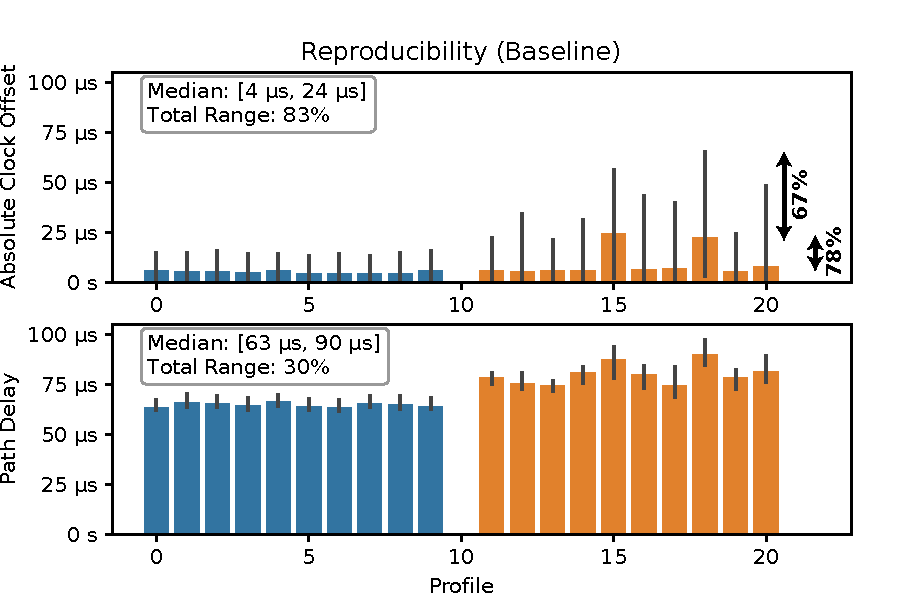
\includegraphics[width=\linewidth]{res/generated/base/key_metric_variance.pdf}
    \caption{Validating the baseline results by repeatedly measuring the baseline for both vendors on the Raspberry Pi 4 system. Top: The median absolute clock offset for each run, with error bars reaching from quantiles 0.05 to 0.95. Bottom: The same for the estimated path delay.}
    \label{fig:baseline_reproducibility}
\end{figure}

\newcommand{\numBaselineMeasurements}{10}
\newcommand{\baselineMinutesRuntime}{\numBaselineMeasurements*4*2*20}

The next question to be answered is how reproducible the baseline is. To evaluate this, we repeat the measurement of the baseline observations ten times for each vendor on each hardware platform (totaling in around \fpeval{round(\baselineMinutesRuntime/60)} hours of runtime and \fpeval{round(\baselineMinutesRuntime*60)} samples collected) and aggregate them. Between each measurement run, the entire cluster is restarted to ensure that no state is carried over, which would harm the independence of observations. Otherwise, the setup is left untouched and all that happens is that the PTP installation is started and stopped.

%Figure \ref{fig:baseline_reproducibility} shows the results. We observe that LinuxPTP produces significantly more stable results for both the clock offset estimation and the path delay, while PTPd shows more variance in median and 95-th quantile observed clock offset, while additionally being less sure about the path delay. A simple restart can suddenly cause the median latency to jump from the median \fTimeKey{ptpd/median} up to \fTimeKey{ptpd/max}, which corresponds to an increase of \fRatio{\ptpKey{ptpd/max}/\ptpKey{ptpd/median}} not only momentarily, but throughout an entire run. This already comes uncomfortably close to our safety factor of \safetyMargin, and we have not even started stressing the system yet. Fortunately, LinuxPTP produces a lot more stable results, with a smaller range of \fTimeKey{linuxptp/median} and \fTimeKey{linuxptp/max} between the median observed run and the worst observed run corresponding to just \fRelative{\ptpKey{linuxptp/max}/\ptpKey{linuxptp/median}}.



\section{Learnings and Conclusion}
\label{sec:learnings_conclusion}
\label{sec:discussion}
\label{sec:learning}
From our experiments we derive the following learnings and best practices:

\paragraph{Choice of Vendor} We have found there to be substantial synchronization performance and reliability differences between the vendors. While deploying PTPd may be tempting due to its simplicity and maturity, the fact that it can soft-brick the network driver along with its often order of magnitudes slower clock convergence\todo{This should be mentioned explicitly somewhere in the baseline} should be enough of a red flag for projects to steer clear of it (and perhaps its derivatives), even if it can offer comparable accuracy with less effort required for setup (of the tested vendors, it was nevertheless the least accurate). Meta's SPTP was developed specifically with datacenter applications in mind and claims resource consumption advantages, however at the time of writing it comes with some limitations (the reduction in data and packet rates appears to be a tradeoff with higher ROM, RAM and compute usage), and most importantly a lack of maturity due to the recent release (this can be easily confirmed by a quick inspection of the documentation). This leaves LinuxPTP for PTP and Chrony as the NTP alternative -- perhaps surprisingly, Chrony appears to outperform LinuxPTP in terms of synchronization quality on our system. However, Chrony requires several times more ROM space, thus making it more difficult to deploy in resource-constrained environments. In the end, both are quite mature and widely adopted, the better fit ultimately depends on the type of deployment.

\paragraph{Guarding against Resource Contention}
When dealing with resource contention, we observe that network congestion is the primary cause of degradation and that the ideal setup physically separates PTP traffic from application traffic (using e.g. a secondary management network). While certain deployments (e.g. datacenter or industrial IoT) might already feature secondary networks, this solution is often an expensive proposition and embedded deployments might opt for the software solution of traffic prioritization instead. However, setting a DSCP priority is not a cure-all for this case: we have shown that in some of our setups applying prioritization can lead to a considerable decrease in synchronization quality (this anomaly likely depends on the combination of priorities, NIC hardware queues and queuing disciplines, as well as network hardware). Thus, using a software prioritization solution requires proper testing before it can be relied upon. Using the default configuration of no prioritization at all is not recommended, as the 95\textsuperscript{th} percentile clock offset under network load can reach as high as \cmpLoad{net_load_vs_baseline}\fRatio[-2]{\cmpMax} the baseline's 95\textsuperscript{th} percentile. Other resources can also play minor roles in the clock synchronization accuracy (with cache contention and memory bandwidth bottlenecks being the most notable), however they do not get anywhere near the magnitude of network contention.

\paragraph{Resilience against Faults} While the most beneficial piece of hardware support for PTP might seem to be a NIC's hardware timestamping capability to protect against queuing and network delays, it turns out that it is actually more important to have an external clock source available to protect against unexpected conditions when failures occur. We strongly recommend using at least a real-time clock (or a better quality clock source such as GNNS) on the master node (and preferably on slave nodes too) to mitigate inconsistencies that inevitably happen when a node loses its state and therefore its system time. Alternatively, if internet access is available, then the master can import its time from a reliable network source, which achieves the same purpose. In lieu of these solutions (e.g. in isolated embedded settings), careful PTP configuration is necessary, as with the defaults edge cases may occur where clocks differ on the order of magnitude of minutes or years indefinitely, something that cannot be fixed solely by e.g. deploying a failover.

%Lessons learned:
%\begin{itemize}
%    \item Don't use PTP:
%    \begin{itemize}
%        \item Convergence order of magnitude slower
%        \item Faults can bring down entire network interface
%    \end{itemize}
%    \item Prefer physical isolation, prioritization needs to be considered carefully
%    \item Prefer real-time clock (at least on master)
%\end{itemize}

While time synchronization capabilities across packet-switched networks are evolving especially with the advent of TSN, it will probably be some time before we see out-of-the-box synchronization capabilities that are dependable and resilient enough to allow the deployment of synchronization-free distributed algorithms that operate at a timescale of interest to real-time systems while maintaining strict correctness requirements. There are simply too many ways yet to break any bound one might place on a clock signal difference through either bad configuration or hardware limitations. Thus, for the time being, the most reliable way to enforce ordering continues to be manual synchronization as part of a distributed algorithm. However, we invite readers to use the experimental capabilities offered by \toolName{} to evaluate upcoming hardware and software capabilities to determine whether this might change in the future, and we hope that our best practices prove useful for real-world deployments.
\todo{Page limit: 11 pages}

\section{Related Work}
\label{sec:related}

%\todo{I have commented out what looked like the single related work paragraph. It seemed out of place between two PTP paragraphs, which provide the necessary background for this work. We can move the related work to end if it is going to be this short.}
Clock synchronization protocols have been proposed for many different applications including packet-switched networks~\cite{sptp, white-rabbit, time-protocol-flooding, time-protocol-low-power} and their strengths and weaknesses have been evaluated analytically~\cite{clock-synchronization-packet-switched-networks}. Due to the need for dependability, multiple studies have compared how time protocols can fail~\cite{ptp-failures}, how fault tolerance and redundancy can be offered~\cite{fault-tolerant-clock-synchronization-distributed-systems}, and how timing protocols might be attacked by malicious actors~\cite{ptp-internal-attacks, byzantine-ptp}. However, we find that there is a lack of literature collecting empirical findings across implementations and protocols, with an early study~\cite{ntp-vs-ptp} from 2006 focusing on technologies that were available at the time and more recent studies~\cite{time-enough} not incorporating fault-tolerance as a central aspect.


\section{Learnings}
Lessons learned:
\begin{itemize}
    \item Don't use PTP:
    \begin{itemize}
        \item Convergence order of magnitude slower
        \item Faults can bring down entire network interface
    \end{itemize}
    \item Prefer physical isolation, prioritization needs to be considered carefully
    \item Prefer real-time clock (at least on master)
\end{itemize}

\printbibliography

\end{document}
